% \documentclass[handout]{beamer}
\documentclass{beamer}

\mode<presentation> {%
	\usetheme[]{Boadilla}
	\usecolortheme{orchid}
	\setbeamercovered{transparent}
	\setbeamersize{text margin left=0.7cm}
  \setbeamersize{text margin right=0.7cm}
  \setbeamertemplate{enumerate item}[square]
  \setbeamertemplate{enumerate subitem}[circle]
  \setbeamertemplate{enumerate subsubitem}[>]
  \setbeamertemplate{itemize item}[square]
  \setbeamertemplate{itemize subitem}[circle]
  \setbeamertemplate{itemize subsubitem}[>]
}

\usepackage{pstricks}
\usepackage{pst-node}
\usepackage{bm}
\usepackage[utf8]{inputenc}
\usepackage[spanish]{babel}
\usepackage[normalem]{ulem}
\usepackage{times}
\usepackage[T1]{fontenc}
\usepackage{graphicx}
\usepackage{multirow}
\usepackage{pifont}
\usepackage{rotating}
\usepackage{colortbl}
\usepackage{verbatim}
\usepackage{amssymb}


\definecolor{olivegreen}{rgb}{0.0,0.5,0.0}
\definecolor{general}{rgb}{0.9 0.9 1}%
\newrgbcolor{colorsistema}{0 1 1}
\newrgbcolor{colorviolet}{0.9 0.8 1}


\title[Procesamiento de Señales]{Muestreo y reconstrucción de señales \\ en el dominio del tiempo}
\author[J. Chacón, M. J. Gómez] {%
	\textit{Ingeniería Electrónica de Comunicaciones}\\
	\vspace{0.6cm}
	\small Jesús Chacón Sombría \\
  \small María José Gómez Silva%
}%\inst{1}

\institute[DACYA] {%\inst{1}%
	\footnotesize  Departamento de Arquitectura de Computadores y Automática\\
  Universidad Complutense de Madrid
}

\date[Muestreo y reconstrucción] % (optional)
{\footnotesize Curso 2022-2023}%{\today / Master}
\subject{Talks}

\pgfdeclareimage[height=0.75cm]{logo}{ucm}

\usepackage[absolute,overlay]{textpos}
\setlength{\TPHorizModule}{1mm}
\setlength{\TPVertModule}{1mm}
\newcommand{\MyLogo}{%
\begin{textblock}{14}(116.0,0.6)
  \pgfuseimage{logo}
\end{textblock}
}

\makeatletter
\numberwithin{section}{part}
\AtBeginPart{
\beamer@tocsectionnumber=0\relax
\frame{\partpage}
}
\makeatother

\begin{document}

\begin{frame}
  \titlepage
\end{frame}

\newcommand*\oldmacro{}%
\let\oldmacro\insertshorttitle%
\renewcommand*\insertshorttitle{%
 \MyLogo
  \oldmacro\hfill%
}

\AtBeginSection[]
{
  \begin{frame}%<beamer>
    \frametitle{Esquema}
  \small
    \tableofcontents[sectionstyle=show/shaded,subsectionstyle=show/shaded/hide]
  \end{frame}
}

\AtBeginSubsection[]
{
  \begin{frame}%<beamer>
    \frametitle{Esquema}
    \small
   \tableofcontents[sectionstyle=show/shaded,subsectionstyle=show/shaded/hide]
      \end{frame}
}

\begin{frame}\frametitle{Objetivos del tema}
  Entender y caracterizar matemáticamente:
  \begin{itemize}
    \small
    \item Funcionamiento de los conversores A/D y D/A.
    \item Efectos del muestreo periódico de una señal continua:
    \begin{itemize}
      \footnotesize
      \item Aliasing.
      \item Comportamiento en frecuencias de una señal de banda limitada.
      \item Teorema de muestreo (Nyquist-Shannon).
    \end{itemize}
    \item Muestreo de señales discretas
    \item Reconstrucción de la señal continua a partir de una señal discreta
    \begin{itemize}
      \footnotesize
      \item Ideal (Filtro paso-bajo ideal)
      \item Retenedores de diferentes ordenes
    \end{itemize}
    \item Cuantificación y codificación de señales
  \end{itemize}
\end{frame}
\begin{frame}[fragile]\frametitle{Procesamiento de una señal}
  \begin{center}
    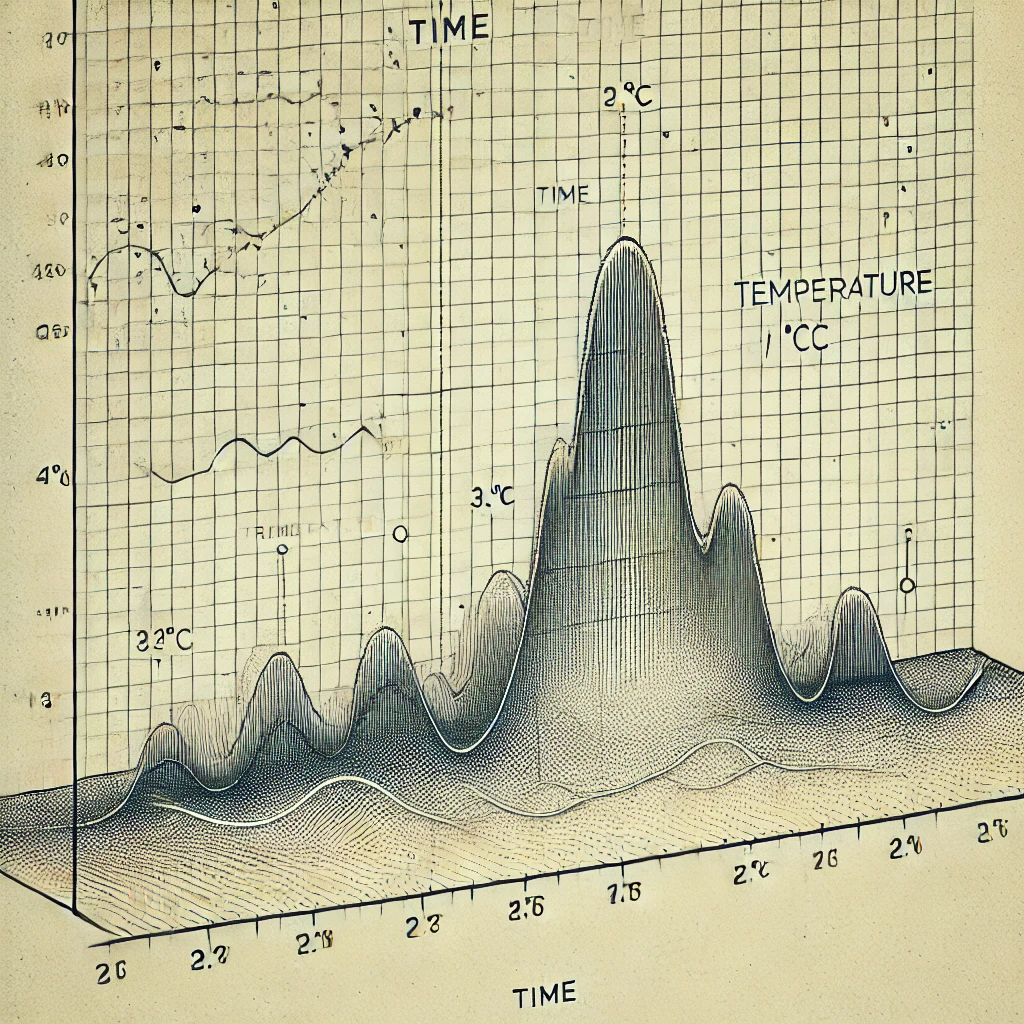
\includegraphics[width=3.5cm]{Figures/TemperatureSignal.png}
    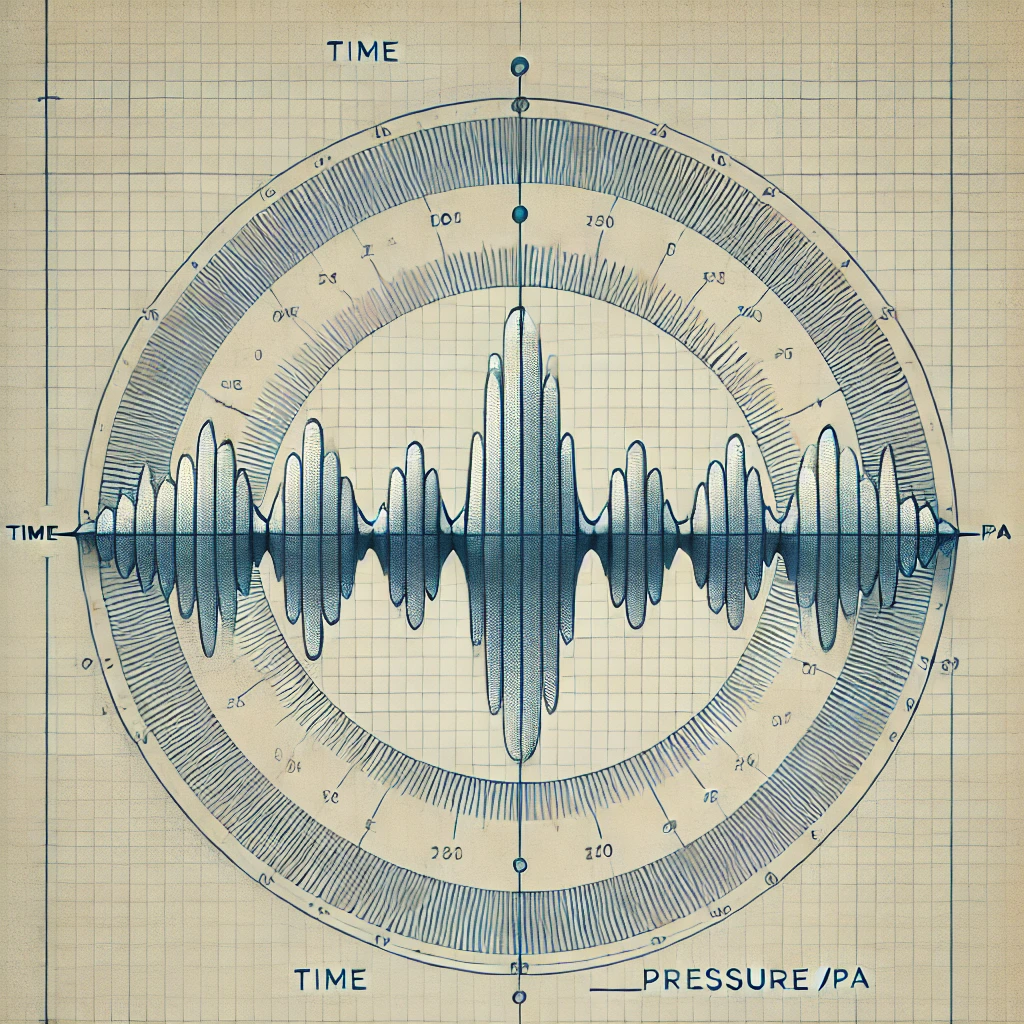
\includegraphics[width=3.5cm]{Figures/SoundPressure.png}
    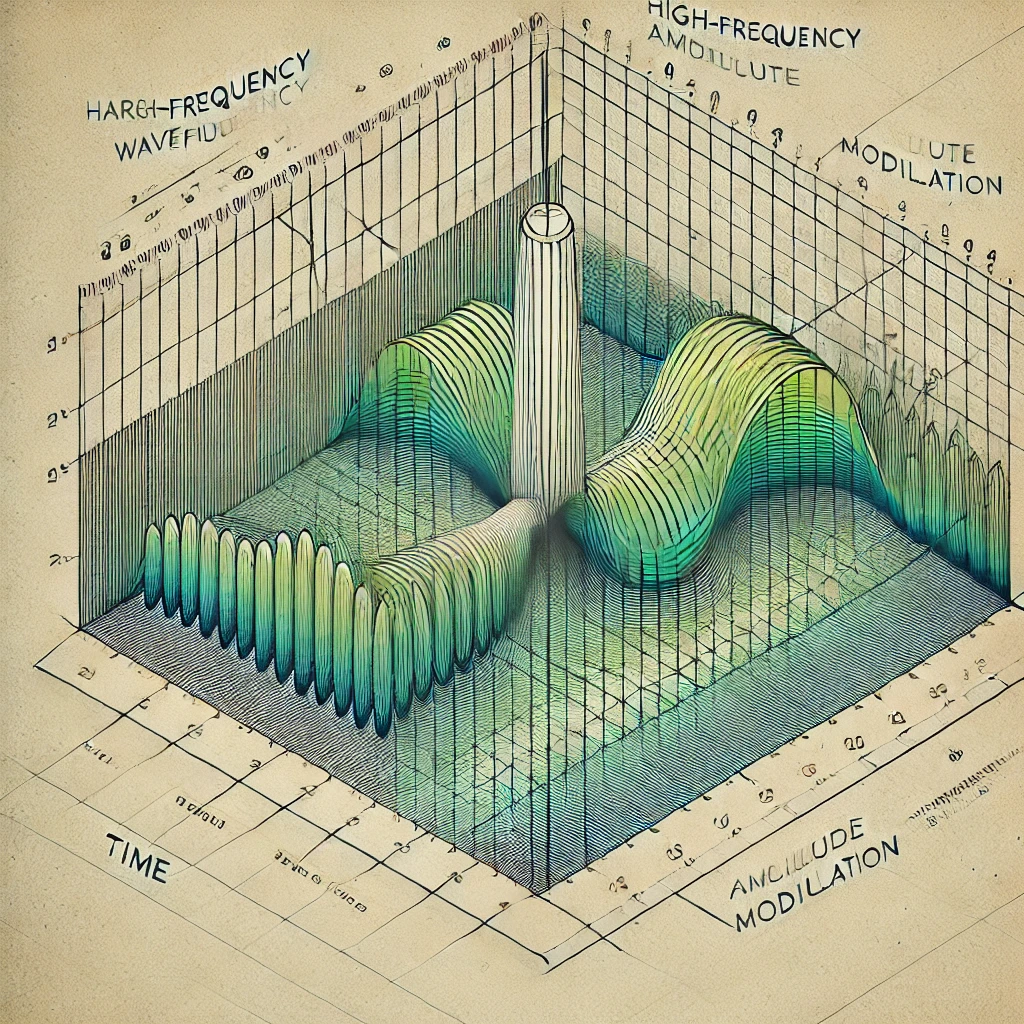
\includegraphics[width=3.5cm]{Figures/Radio.png}
  \end{center}
  \begin{itemize}
    \item Las señales provenientes del mundo real habitualmente son analógicas:
    \begin{itemize}
      \item Temperatura.
      \item Sonido (ondas de presión sonora).
      \item Señales de radio (ondas electromagnéticas).
    \end{itemize}
  \end{itemize}
\end{frame}

\begin{frame}\frametitle{Procesadores de señales}
  \begin{figure}
    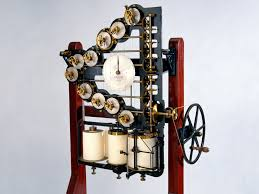
\includegraphics[height=2.5cm]{Figures/mareas.jpg}
    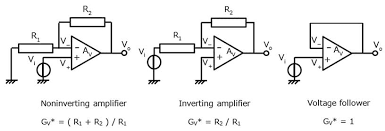
\includegraphics[height=2.5cm]{Figures/opamp.png}
  \end{figure}
  \begin{itemize}
    \item Los primeros procesadores de señales eran analógicos \href{https://www.youtube.com/watch?v=IgF3OX8nT0w}{(ver vídeo)}:
    \begin{itemize}
      \item Predictor de Mareas (Lord Kelvin, 1873).
      \item Moduladores/demodulares para comunicaciones.
      \item Filtros analógicos.
      \item Amplificadores operacionales (1939).
      \begin{itemize}
        \item Operaciones: suma, resta, integración, derivación...
        \item Filtros
      \end{itemize}
    \end{itemize}
    \item Algunas ventajas:
    \begin{itemize}
      \item Velocidad de procesamiento.
    \end{itemize}
    \item Algunas desventajas:
    \begin{itemize}
      \item Sensible al ruido.
      \item Poco flexible.
    \end{itemize}
  \end{itemize}
\end{frame}

\begin{frame}\frametitle{Procesadores de señales}
  \begin{center}
    \begin{tikzpicture}
      % Nodes
      \node (input) [] {};
      \node (adc) [block, right=0.8cm of input] {\tiny A/D};
      \node (dsp) [block, right=0.8cm of adc] {\tiny Procesador digital};
      \node (dac) [block, right=0.8cm of dsp] {\tiny D/A};
      \node (output) [right=0.8cm of dac] {};
      % Arrows
      \draw [arrow] (input) -- (adc) node[midway, above] {\tiny $x(t)$};
      \draw [arrow] (adc) -- (dsp) node[midway, above] {\tiny $x_d[n]$};
      \draw [arrow] (dsp) -- (dac) node[midway, above] {\tiny $y_d[n]$};
      \draw [arrow] (dac) -- (output) node[midway, above] {\tiny $y_a(t)$};
    \end{tikzpicture}
  \end{center}
  \begin{itemize}
    \item El auge de la electrónica digital plantea un enfoque alternativo.
    \begin{itemize}
      \item Convertir la señal continua en discreta mediante el muestreo.
      \item Procesar digitalmente.
      \item Reconstruir una señal continua a partir de las muestras procesadas. 

    \end{itemize}
    \item Algunas ventajas:
    \begin{itemize}
      \item Mayor flexibilidad.
      \item Menos sensible al ruido.
    \end{itemize}
    \item Algunas desventajas:
    \begin{itemize}
      \item Menor velocidad/latencia.
      \item Rango dinámico limitado.
    \end{itemize}
  \end{itemize}
\end{frame}

\begin{frame}\frametitle{Procesadores de señales}
  \begin{center}
    \begin{tikzpicture}
      % Nodes
      \node (input) [] {};
      \node (adc) [block, right=0.8cm of input] {\tiny A/D};
      \node (dsp) [block, right=0.8cm of adc] {\tiny Procesador digital};
      \node (dac) [block, right=0.8cm of dsp] {\tiny D/A};
      \node (output) [right=0.8cm of dac] {};
      % Arrows
      \draw [arrow] (input) -- (adc) node[midway, above] {\tiny $x(t)$};
      \draw [arrow] (adc) -- (dsp) node[midway, above] {\tiny $x_d[n]$};
      \draw [arrow] (dsp) -- (dac) node[midway, above] {\tiny $y_d[n]$};
      \draw [arrow] (dac) -- (output) node[midway, above] {\tiny $y_a(t)$};
    \end{tikzpicture}
  \end{center}
  \begin{itemize}
    \item Procesamiento digital de señales
    \begin{itemize}
      \item Algunos hitos históricos:
      \begin{itemize}
        % \item 1805 - Gauss (\emph{¡Cómo no!}): algoritmo precursor de la FFT\footnote{Aunque no lo publico en vida, según investigaciones recientes se le atribuye a Gauss (\emph{¡Cómo no!}) un algoritmo para el cálculo de coef. de SF finitas considerado el precursor de lo que hoy conocemos como FFT.}
        \item 1807, 1811 - Publicación resultados sobre series de Fourier\footnote{Según investigaciones recientes se le atribuye a Gauss (\emph{¡Cómo no!}), aunque no lo publico en vida, un algoritmo para el cálculo de coef. de SF finitas considerado el precursor de lo que hoy conocemos como FFT.}
        % \item 1821 - Primer ordenador digital: máquina diferencial de \emph{Babbage}
      %   % \item 1946 - ENIAC \emph{Electrical Numerical Integrator and Calculator}
        % \item 1947 - Invención del transistor (\emph{Bardeen}, \emph{Brattain} y \emph{Shockley})
        \item 1965 - Cooley \& Tukey: algoritmo FFT (Fast Fourier Transform)
        \item 1978 - INTEL lanza el 2920: procesador de señales analógicas
        \item 1982 - Texas Instruments lanza el TMS32010\\
        \hspace{1cm}{\scriptsize Primer procesador digital de señales (DSP) propiamente dicho}\\
        \hspace{1.5cm}{\scriptsize \color{blue}$\bullet$ \color{black} Arquitectura Harvard: datos e instrucciones separados}\\
        \hspace{1.5cm}{\scriptsize \color{blue}$\bullet$ \color{black} Operaciones MAC (Multiply-Accumulate)}\\
      \end{itemize}
    \end{itemize}
  \end{itemize}
\end{frame}


\begin{frame}[fragile]\frametitle{Procesador Digital de Señales (DSP)}
  \begin{tikzpicture}
    % Nodes
    \node (input) [] {};
    \node (antialiasing) [block, right=1cm of input] {\begin{minipage}{1.25cm}\centering\setlength{\baselineskip}{1.5em}\tiny Filtro\\ anti-aliasing\end{minipage}};
    \node (adc) [block, right=0.8cm of antialiasing] {\tiny A/D};
    \node (dsp) [block, right=0.8cm of adc] {\tiny Procesador digital};
    \node (dac) [block, right=0.8cm of dsp] {\tiny D/A};
    \node (smoothing) [block, right=0.8cm of dac] {\begin{minipage}{1.25cm}\centering\setlength{\baselineskip}{1.5em}\tiny Filtro de\\suavizado\end{minipage}};
    \node (output) [right=0.8cm of smoothing] {};
    % Arrows
    \draw [arrow] (input) -- (antialiasing) node[midway, above] {\tiny $x(t)$};
    \draw [arrow] (antialiasing) -- (adc) node[midway, above] {\tiny $x_a(t)$};
    \draw [arrow] (adc) -- (dsp) node[midway, above] {\tiny $x_d[n]$};
    \draw [arrow] (dsp) -- (dac) node[midway, above] {\tiny $y_d[n]$};
    \draw [arrow] (dac) -- (smoothing) node[midway, above] {\tiny $y_a(t)$};
    \draw [arrow] (smoothing) -- (output) node[midway, above] {\tiny $y(t)$};
  \end{tikzpicture}
  \begin{itemize}
    \item \alert{Esquema general:}
    \begin{itemize}\scriptsize
      \item El filtro antialiasing garantiza una señal de ancho de banda limitado.
      \item El ADC convierte la señal analógica en una señal digital.
      \item El procesador digital realiza la manipulación de la señal.
      \item El DAC convierte la señal digital en una señal analógica.
      \item El filtro de suavizado elimina las altas frecuencia debidas a la reconstrucción.
    \end{itemize}
  \end{itemize}
\end{frame}


\begin{frame}\frametitle{Muestreo, cuantificación y codificación}
  \footnotesize
  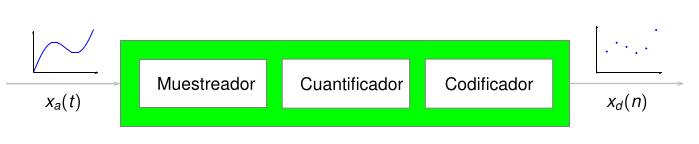
\includegraphics[width=\textwidth]{Figures/MCC.png}
  \begin{itemize}
    \item \textbf{Muestreo}: Es la conversión de una señal analógica $x_a(t)$ en una señal de tiempo discreto x(n). Consiste en tomar ``muestras'' de la señal continua $x_a(t)$ en ciertos instantes de tiempo: $x(n)=x_a(t=t_n)$.
    \item \textbf{Cuantificación}\visible<5->{$^{1}$}: Es la conversión de una señal de tiempo discreto $x(n)$ que toma valores continuos en una señal de tiempo discreto que toma también valores discretos, es decir en una señal digital $x_d(n)$.
    \item \textbf{Codificación}: Cada valor digital $x_d(n)$ se representa mediante una secuencia binaria \{011011101010101\}.
  \end{itemize}
  \rule{5cm}{0.4pt}\scriptsize\\
  $^1$ El muestreo y la cuantificación pueden realizarse en orden inverso. En la práctica siempre se realizan asi. 
\end{frame}



\begin{frame}\frametitle{Muestreo periódico}
  \small
  \begin{itemize}
    \item Existen diferentes métodos para muestrear una señal continua $x_c(t)$
    \vspace{0.0cm}
    \visible<2->{
    \item Sin embargo, el más común es el \alert{muestreo periódico} o uniforme:}\\
    \vspace{0.1cm}
    \visible<2->{
    \hspace{2cm} \alert{$t=nT_s$ \hspace{1cm}  $\rightarrow$
    \hspace{1cm} $x_d(n)=x_c(nT_s)$}}
    \vspace{-0.1cm}
    \begin{columns}[c]
      \hspace{0.5cm}\begin{column}{4cm}
        \vspace{0.3cm}
        \only<1-2|handout:0>{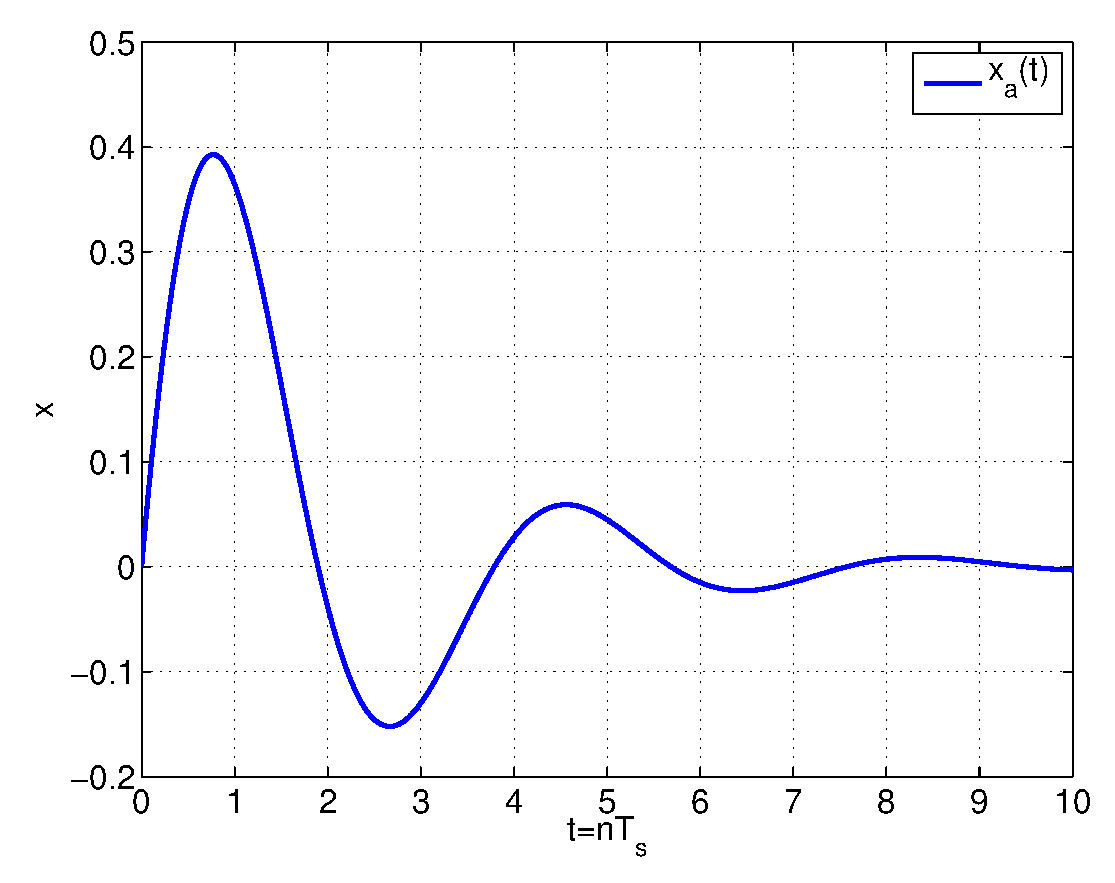
\includegraphics[width=4.5cm]{./Figures/Muestreo1.eps}}
        \only<3->{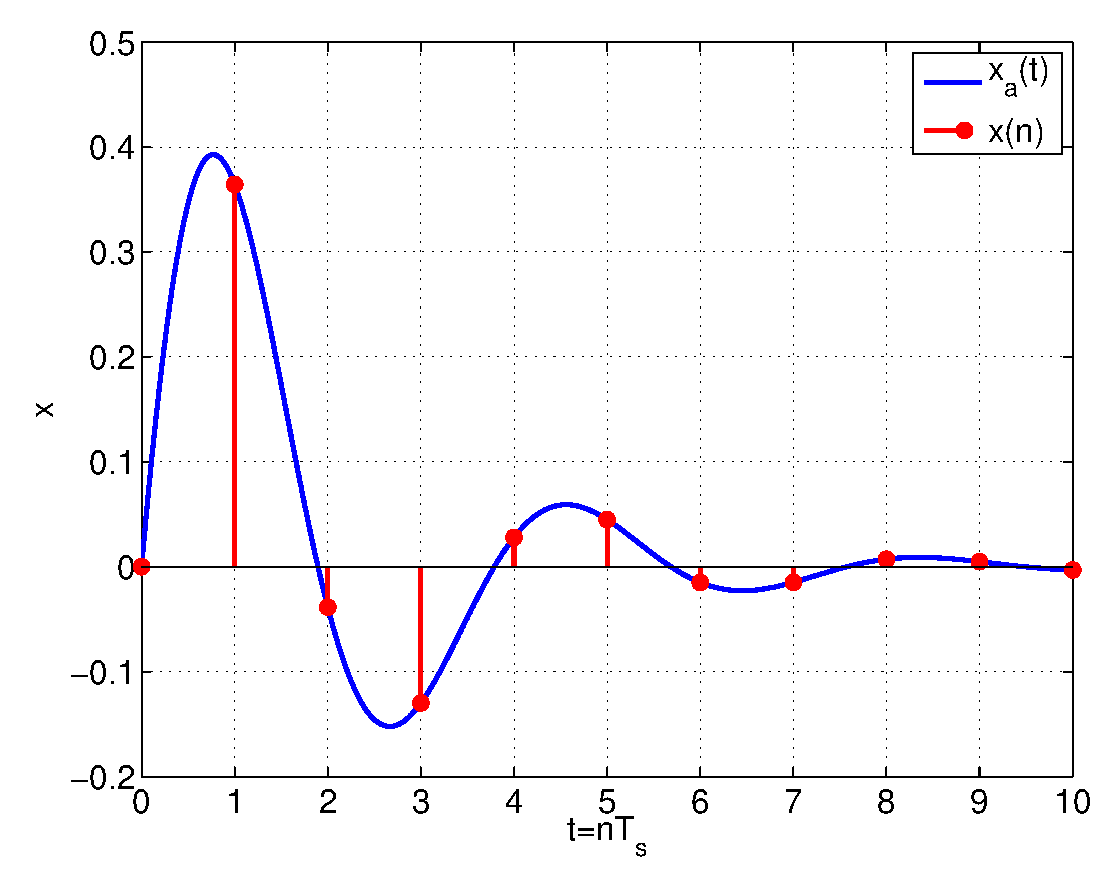
\includegraphics[width=4.5cm]{./Figures/Muestreo2.eps}}
      \end{column}
      \hspace{-0.5cm}\begin{column}{6cm}
        \visible<4->{
        \begin{itemize}
        \item El tiempo $T_s$ entre dos muestras es constante y se llama periodo de muestreo.
        \item $F_s=\frac{1}{T_s}$ se llama frecuencia de muestreo.
        \item Como las variables $t$ (tiempo continuo) y $n$ (tiempo discreto) están relacionadas por $t=nT_s$,
        \end{itemize}}
      \end{column}
    \end{columns}
    \visible<4->{
    para muestrear de forma periódica cualquier señal continua $x_c(t)$ basta con evaluarla en los instantes de muestreo $x_d(n)=x_c(nT_s)$}
  \end{itemize}
  \visible<5->{
  \hrule
  \vspace{0.2cm}
  \color{gray}
  \footnotesize
  La señal muestreada se puede representar respecto a $n$ o a $T_s n$.}
\end{frame}


\begin{frame}\frametitle{Muestreo y reconstrucción}
  \begin{itemize}
    \item \alert{Analizamos un caso sencillo:}
    \begin{itemize}
      \item<1-> Muestreamos $x(t)=cos(\omega_0 t)$ con un periodo $T_s$ (\color{blue}$t=nT_s$\color{black}).
      \item<2-> ¿Como elegimos el valor de $T_s$? ¿Qué importancia tiene?
      \item<3-> La versión discreta de $x(t)$ es \color{blue}$x_d[n]=cos(\omega_0 T_s n)$\color{black}.
    \end{itemize}
    \item \alert{¿Qué ocurre al pasar del mundo continuo al discreto?}
    \begin{itemize}
      \item Recordemos que, en continuo, $\omega_1\neq\omega_2 \Rightarrow cos(\omega_1 )\neq cos(\omega_2 t)$.
      \item Sin embargo, en discreto para $k=0,1,2,3,...~$:
      \color{blue}\[\omega_k = \omega_0 T_s + 2\pi k \Rightarrow cos(\omega_k n) = cos(\omega_0 T_s n)\]
    \end{itemize}
  \end{itemize}
  \begin{alertblock}{Fenómeno de aliasing}
    \centering Existen infinitas señales continuas que, al muestrear con periodo $T_s$, generan la misma secuencia de muestras.
  \end{alertblock}
\end{frame}

\begin{frame}\frametitle{Muestreo y reconstrucción}
  \begin{itemize}
    \item \alert{¿Por qué se denomina \emph{aliasing}?}
    \begin{itemize}
      \item<1-> Cada una de las frecuencias continuas \color{blue}$\omega_k=\omega_0 + \frac{2\pi}{T_s} k$ \color{black} es un \color{blue}\emph{alias}\color{black}.
      \item<2-> Si $|\omega Ts|> \pi$, entonces $|\omega Ts - 2\pi k|\geq\pi$ para algún $k$.
      \item<3-> Es decir, existe una señal de frecuencia más baja que genera las misma secuencia de muestras para el periodo de muestreo $T_s$.
    \end{itemize}
  \end{itemize}
  \begin{alertblock}{Alias fundamental}
    \centering Llamamos \color{blue}\emph{alias fundamental} \color{black}a la señal de frecuencia más baja ($\omega_0$) de entre las que generan la misma secuencia de muestras ($x[n]$).
  \end{alertblock}
\end{frame}

\begin{frame}\frametitle{Ejemplos de aliasing en señales sinusoidales I}
  \small\hspace{1.9cm}\alert{$x_d(n)=x_c(nT_s)=sen(w_cT_sn+\phi)=sen(w_dn+\phi)$}
  \vspace{-0.1cm}
  
  \begin{itemize}
    \footnotesize
    \item \color{olivegreen} ¿Cual es el alias fundamental de  $x_c(t)=sen(\frac{2\pi}{10}t)$ cuando el periodo de muestreo es de 2s? \color{gray}\\
    \vspace{0.1cm}$w_d=\frac{2\pi}{10} \cdot 2=\frac{4\pi}{10}$.\\
    \vspace{0.1cm}Como $|w_d|<\pi$ ya tenemos el alias fundamental.
  \end{itemize}

  \vspace{-0.5cm}
  \begin{columns}[c]
    \begin{column}{6.8cm}\footnotesize
      \begin{itemize}
        \item \color{olivegreen} ¿Cual es el alias fundamental de $x_c(t)=sen(\frac{2\pi}{10/6}t)$ cuando el periodo de muestreo es de $2s$ \color{gray}\\
        $w_d=\frac{2\pi}{10/6} \cdot 2=\frac{24\pi}{10}$.\\
        Como $|w_d|>\pi$ tenemos que obtener el alias fundamental.\\
        $w_{d2}=\frac{24\pi}{10}-2\pi=\frac{4\pi}{10}$.\\
        $w_{c2}=w_{d2}/T_s=\frac{2\pi}{10}$. Por lo tanto, el alias fundamental es el que se obtiene en la tarea anterior.  
      \end{itemize}
    \end{column}\hspace{-0.4cm}
  \begin{column}{4.5cm}
  {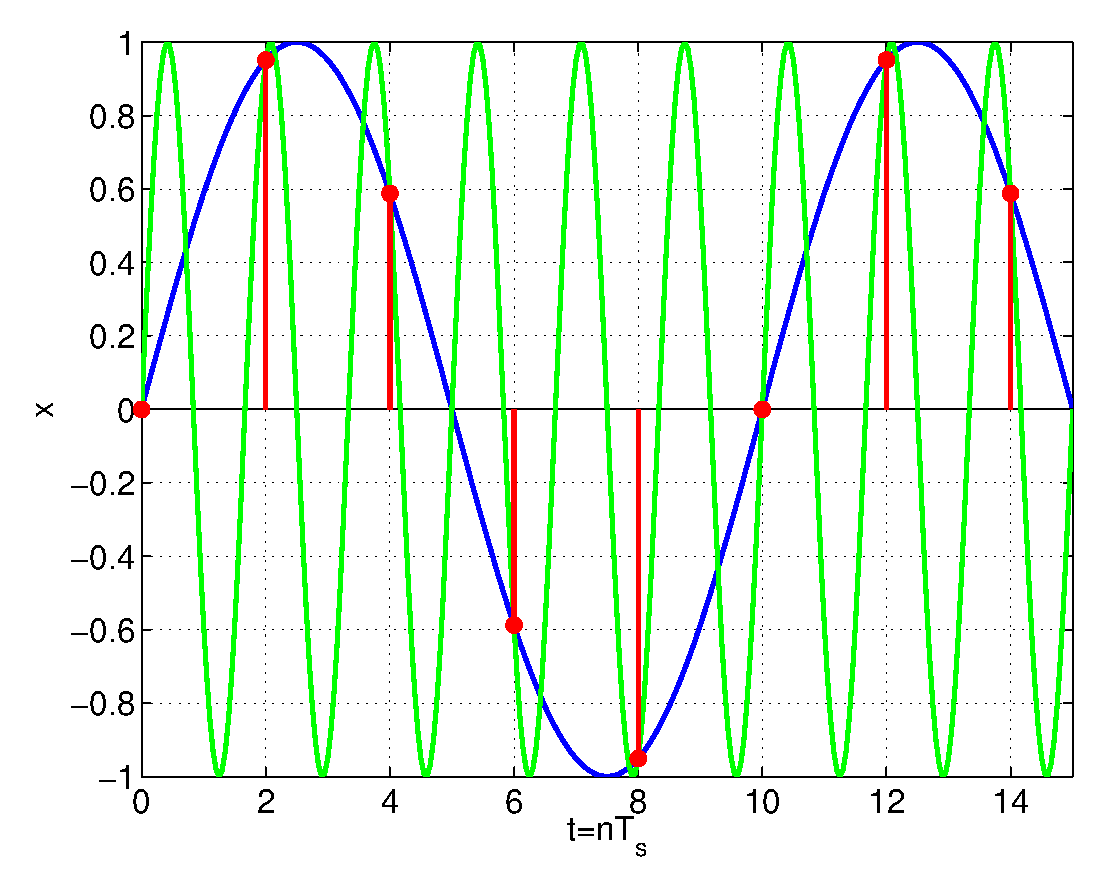
\includegraphics[width=4.5cm]{./Figures/AliasBasic3.eps}}
    \end{column}
  \end{columns}
\end{frame}

\begin{frame}\frametitle{Ejemplos de aliasing de señales sinusoidales II}\small
  \hspace{1.9cm}
  \alert{$x_d(n)=x_c(nT_s)=sen(w_cT_sn+\phi)=sen(w_dn+\phi)$} 
  \vspace{-0.1cm} 
  \begin{itemize}\footnotesize
    \item \color{olivegreen} ¿Cual es el alias fundamental de $x_c(t)=3 sen(\frac{2\pi}{5}t)+ sen(\frac{2\pi}{3}t)$ cuando se muestrea con un periodo de 2s? \color{gray}
  \end{itemize}

  \begin{columns}[c]
    \begin{column}{4.6cm}
      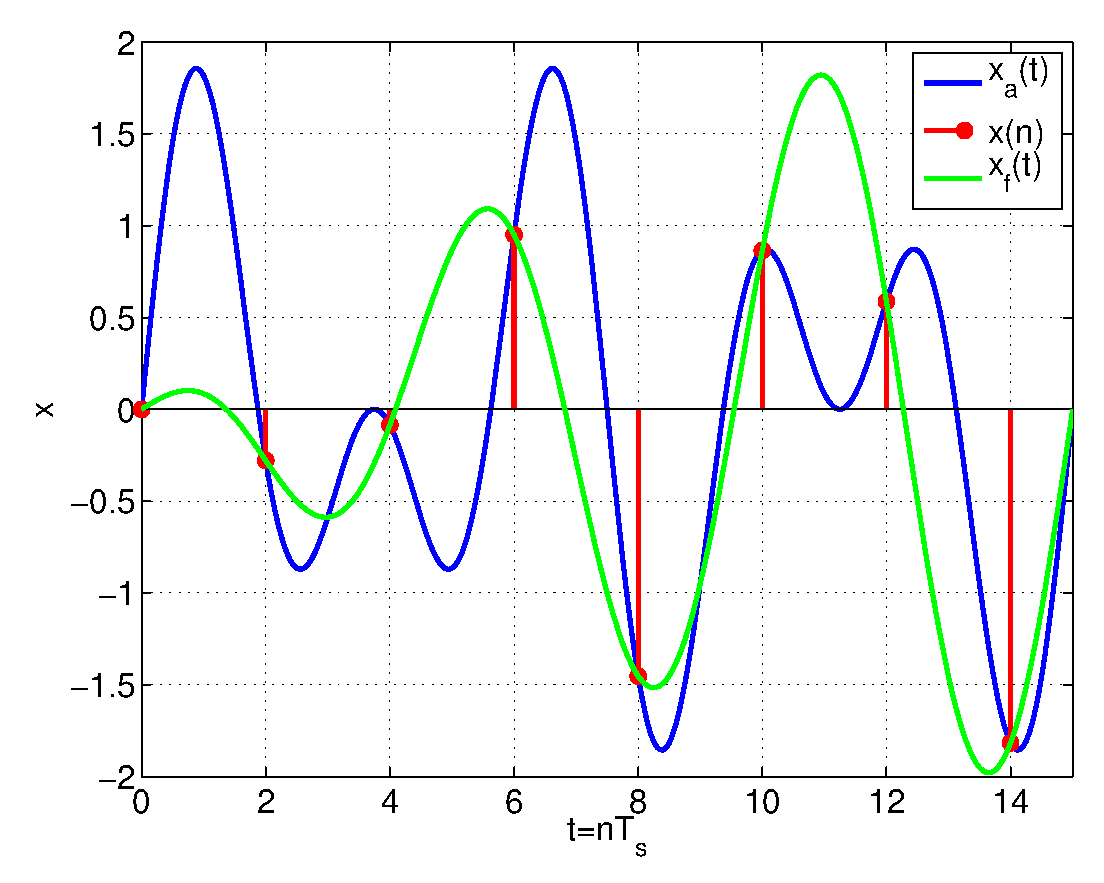
\includegraphics[width=4.5cm]{./Figures/AliasEj3_2.eps}
    \end{column}
    \begin{column}{6.2cm}\color{gray}\footnotesize
      $w_{c1}=\frac{2 \pi}{5}$ $\rightarrow w_{d1}=\frac{4 \pi}{5}$\\
      \vspace{0.1cm}
      $w_{c2}=\frac{2 \pi}{3}$ $\rightarrow  w_{d2}=\frac{4 \pi}{3}$\\
      \vspace{0.1cm}  
      $|w_{d1}|<\pi$. No hay que calcular su alias fundamental.\\
      \vspace{0.1cm}
      $|w_{d2}|>\pi$. Hay que calcular su alias fundamental.\\
      \vspace{0.1cm}
      $w'_{d2}=\frac{4 \pi}{3}-2\pi=\frac{-2 \pi}{3}$
      \vspace{0.1cm}
      $w'_{c2}=\frac{w'_{d2}}{T_s}=\frac{- \pi}{3}$
      \vspace{0.1cm}
      $x'_c(t)=3 sen(\frac{2\pi}{5}t)+ sen(\frac{-\pi}{3}t)$
      \vspace{0.1cm}
    \end{column}
  \end{columns}
\end{frame}

\begin{frame}\frametitle{Muestreo y reconstrucción}
  {\hspace{0.8cm} \alert{¿Es posible reconstruir totalmente una señal muestreada?} }
  \vspace{0.2cm}
  \visible<4->{
  \hspace{5cm}\alert{¿$x_a(t)=y_a(t)$?}}
  \vspace{0.3cm}
  \begin{columns}[T]
    \begin{column}{5cm}\footnotesize
      \alert{De forma general, no es posible.}\\
      \vspace{0.3cm} 
      Sin embargo en algunos casos se puede reconstruir idealmente la señal o una señal muy parecida.
    \end{column}
    \begin{column}{5cm}
      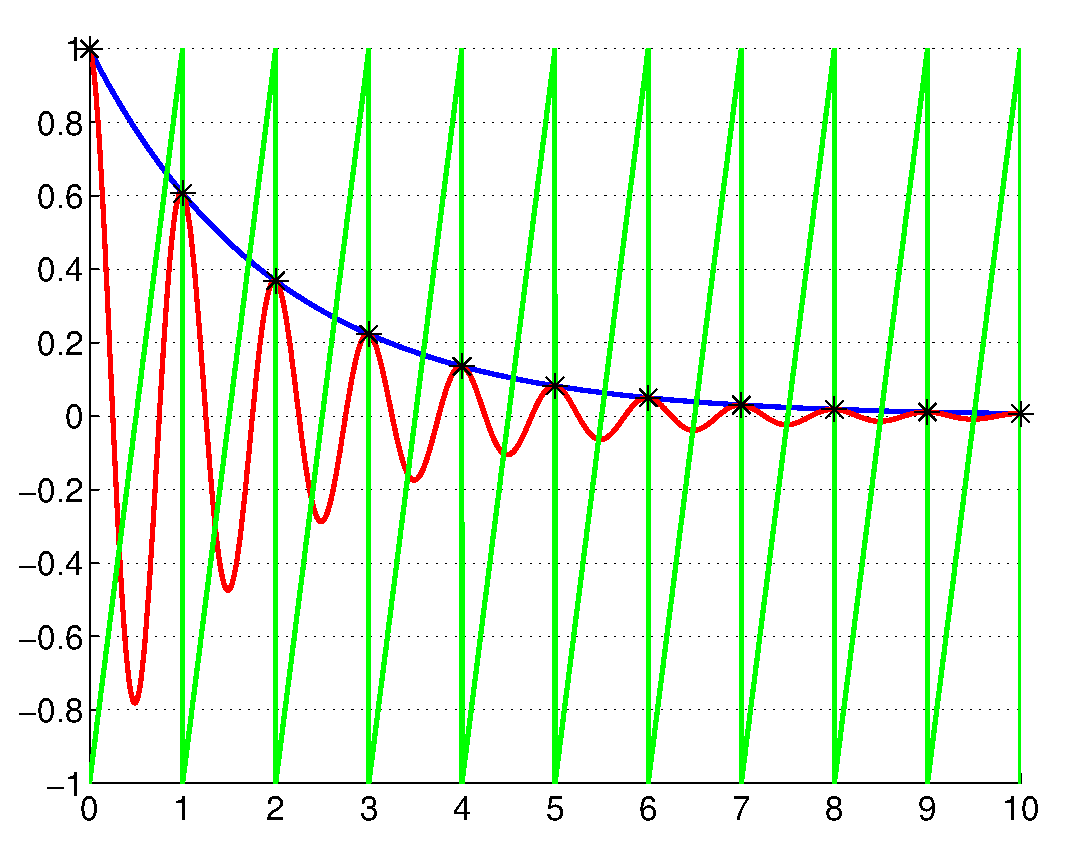
\includegraphics[width=4cm]{./Figures/MuestreoRec4.eps}
    \end{column}
  \end{columns}
\end{frame}

\begin{frame}\frametitle{Análisis en frecuencia del muestreo}
  \begin{block}{Propiedad de muestreo de $\delta(t)$}
    \centering$x(t_0)=\int_{-\infty}^{\infty}x(\tau)\delta(t_0-\tau)d\tau~\quad~x(t)=\int_{-\infty}^{\infty}x(\tau)\delta(t-\tau)d\tau$
  \end{block}
  \alert{Caracterización del muestreo mediante $\delta(t)$}
  \begin{itemize}
    \item Representamos el proceso de muestrear periódicamente una señal mediante un tren de impulsos $p(t)=\substack{\infty\\\sum\\n=-\infty}{\delta(t-n T_s)}$. 
    \item Entonces, la señal muestreada es \[x_d(t)=x(t)p(t)=\substack{\infty\\\sum\\n=-\infty}{x(t)\delta(t-n T_s)}\]
  \end{itemize}
  \begin{alertblock}{Visión continua del muestreo}\centering
    Aunque $x_d(t)$ es la versión muestreada de $x(t)$, es importante\\recalcar que $x_d(t)$ sigue siendo una señal de tiempo continuo.
  \end{alertblock}
\end{frame}

\begin{frame}\frametitle{Análisis en frecuencia del muestreo}
  \begin{block}{Recuerda...}
    \begin{itemize}
      \item Transformada de Fourier de una señal periódica\\[0.5ex]
    $c[k]=\frac{1}{T}\int_T x(t)\mathrm{e}^{-\frac{2\pi}{T} k t}dt \Rightarrow$
    $X(\omega)=\substack{\infty\\\sum\\n=-\infty} 2\pi c[k]\delta(\omega- k \frac{2\pi}{T})$
    \item Propiedad de convolución\\[0.5ex]
    $x_d(t)=x(t)p(t)~\Rightarrow~X(\omega)=\frac{1}{2\pi}\int_{-\infty}^{\infty}{X_d(\Omega)P(\omega - \Omega)}d\Omega$
    \end{itemize}
  \end{block}

  \begin{itemize}
    \item El tren de impulsos es una señal periódica con periodo $T_s$.
    \item Su desarrollo en CFS es: $c[k]=\frac{1}{T_s}\int_{-T_s/2}^{T_s/2}\delta(t)\mathrm{e}^{\frac{2\pi}{T_s} k t}dt=\frac{1}{T_s}$
    \item Su transformada de Fourier es \color{blue}$P(\omega)=\substack{\infty\\\sum\\n=-\infty}\frac{2\pi}{T_s}\delta(\omega- k \frac{2\pi}{T_s})$\color{black}
  \begin{alertblock}{La TF del tren de impulsos es otro tren de impulsos}\centering
    $\substack{\infty\\\sum\\n=-\infty}\delta(t - n T_s) \Leftrightarrow
    \frac{2\pi}{T_s}\substack{\infty\\\sum\\n=-\infty}\delta(\omega- k \frac{2\pi}{T_s})$
  \end{alertblock}
  \end{itemize}
\end{frame}

\begin{frame}\frametitle{Análisis en frecuencia del muestreo}
  \begin{itemize}
    \item Entonces, la CTFT de la señal muestreada es: \[X_d(\omega)=\frac{1}{2\pi}\int_{-\infty}^{\infty}X(\omega - \Omega)P(\Omega)d\Omega=\frac{1}{T_s}\substack{\infty\\\sum\\n=-\infty}X(\omega- k \frac{2\pi}{T_s})\]
    \item Convolución del espectro de la señal original y el tren de impulsos.
  \end{itemize}
  \begin{alertblock}{El espectro se escala y se replica infinitas veces}
    \vspace{0.2cm}
    \[X_d(\omega)=\frac{1}{T_s}\substack{\infty\\\sum\\n=-\infty}X(\omega- k \frac{2\pi}{T_s})\]
    \vspace{0.1cm}
  \end{alertblock}
\end{frame}

\begin{frame}\frametitle{Conceptos importantes}
  \begin{itemize}
    \item \alert{Diferencia entre procesamiento analógico y digital}
    \item \alert{Procesador de Señales Digitales (DSP)}
    \begin{itemize}
      \item Esquema y componentes
      \item Necesidad de muestreo y reconstrucción
    \end{itemize}
    \item \alert{Muestreo periódico}
    \begin{itemize}
      \item Fenómeno de aliasing
      \item Análisis en frecuencia del muestreo
    \end{itemize}
  \end{itemize}
\end{frame}
% \subsection{Señales de banda limitada}

% \begin{frame}
% \frametitle{Análisis en frecuencia del muestreo ideal I}

% \begin{columns}[c]
% \begin{column}{7cm}
% \footnotesize


% \begin{itemize}


% \item \alert{Suponemos que tenemos una señal continua $x_c(t)$ de banda en frecuencia limitada ($X_c(jw)=0$ para $|w|>w_M$)}

% \vspace{0.5cm}

% \visible<2->{

% \item Vamos a realizar el análisis en frecuencia de la señal muestreada, teniendo en cuenta el espectro de la señal continua. }

% \begin{itemize}

% \footnotesize

% \vspace{-0.1cm}
% \visible<3->{
% \item Señal discreta: $x_d(n)=x_c(T_sn)$

% \vspace{0.2cm}}

% \visible<4->{
% \item Visión continua de la señal discreta (\alert{muestreo ideal, a través de la $\delta(\cdot)$}):

% \vspace{0.2cm}
% \hspace{0.5cm}	$x_p(t)\!=\!\sum_{k=-\infty}^{\infty}\!x_c(t)\delta(t-kT_s)\!=$

% \vspace{0.2cm}
% \hspace{1.2cm}	$=\!x_c(t)\!\cdot \! \sum_{k=-\infty}^{\infty}\! \!\delta(t-kT_s)=$

% \vspace{0.2cm}
% \hspace{1.2cm}	$\!=\!x_c(t)\!\cdot\! p(t)$
% }

% \end{itemize}
% \end{itemize}
% \end{column}
% \begin{column}{5cm}
% \vspace{-0.3cm}
% 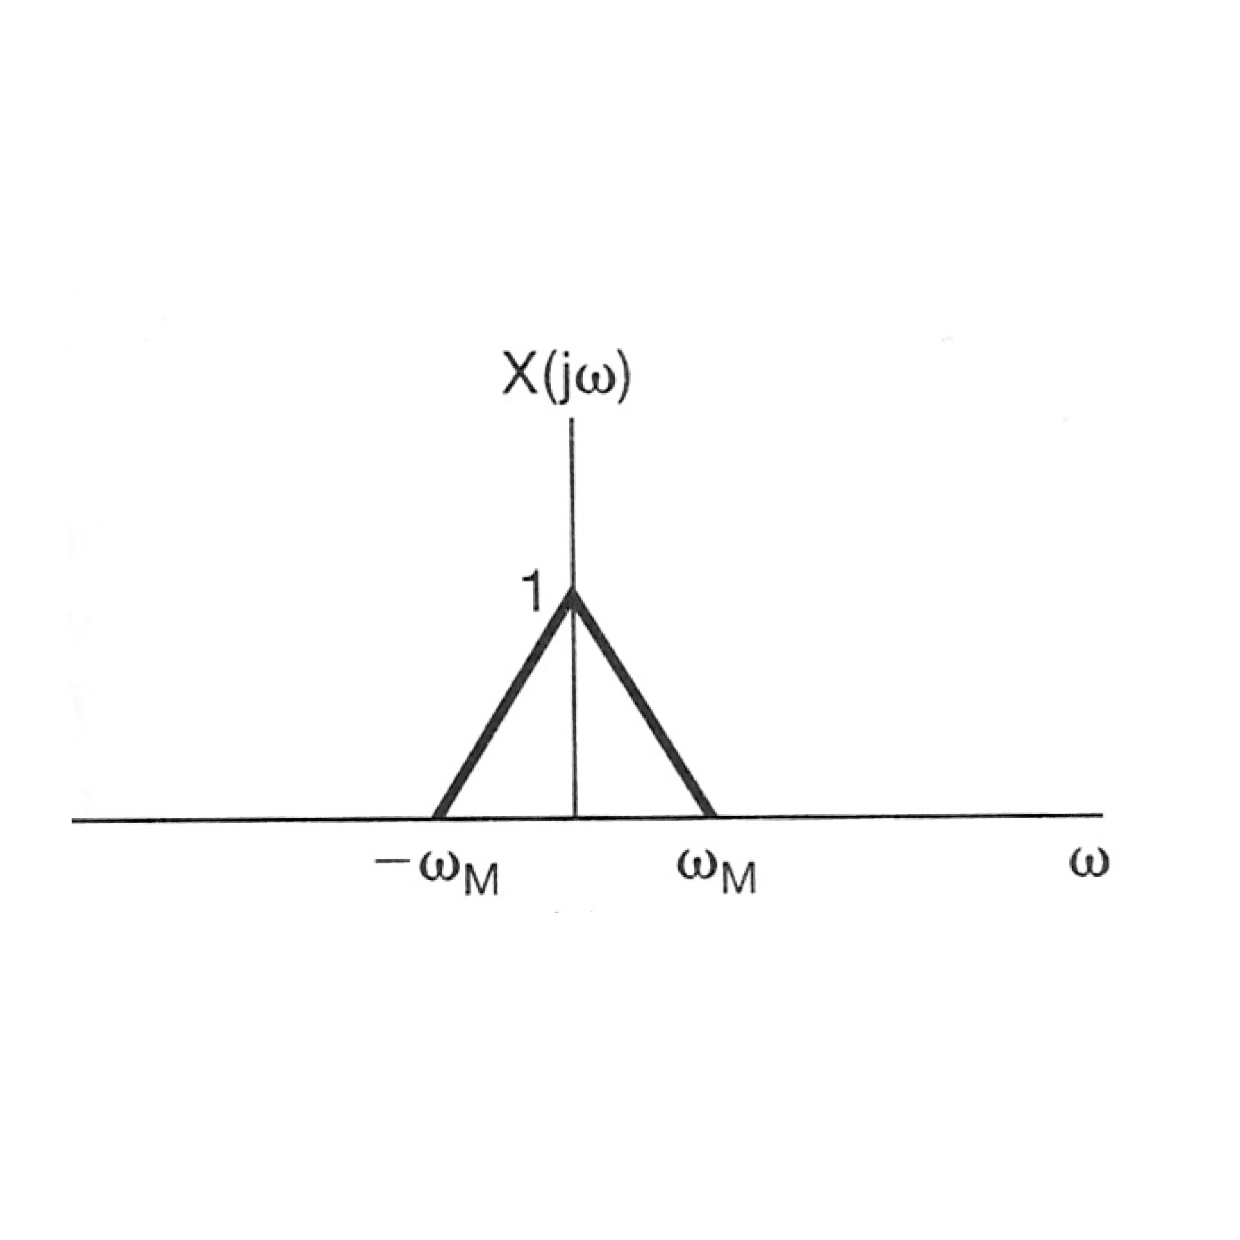
\includegraphics[width=5cm]{./Figures/Muestreo0.ps}
% \vspace{-1.5cm}
% \visible<3->{
% 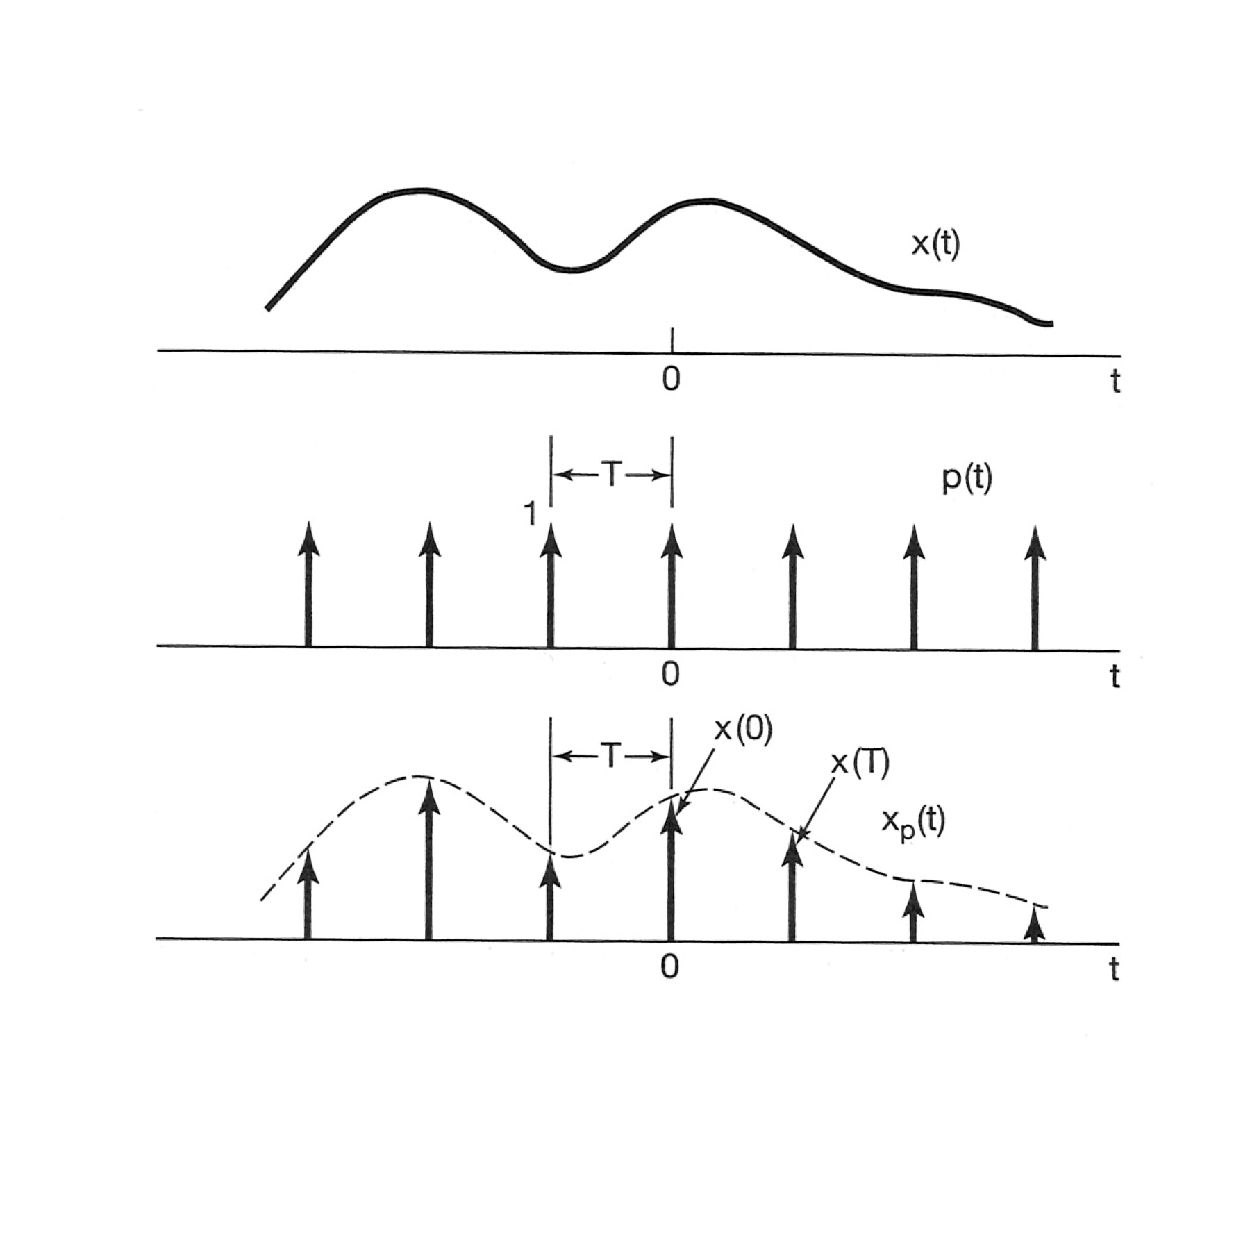
\includegraphics[width=5cm]{./Figures/Muestreo1.ps}}
% \end{column}
% \end{columns}
% \end{frame}

% %%%%%%%%%%%%%%%%%%%%%%%%%%%%%%%%%%%%%%%


% \begin{frame}
% \frametitle{Análisis en frecuencia del muestreo ideal II}

% \footnotesize

% \begin{itemize}
% \item \alert{Señal continua $x_c(t)$ de banda limitada ($X_c(jw)=0$ para $|w|>w_M$)}

% \color{gray}
% \item Análisis en frecuencia de la señal muestreada:

% \begin{itemize}

% \color{gray}
% \footnotesize

% \vspace{-0.1cm}
% \visible<1->{
% \item Señal discreta: $x_d(n)=x_c(T_sn)$

% \vspace{0.1cm}}

% \visible<1->{
% \item Visión continua de la señal discreta (\alert{muestreada idealmente $\delta(\cdot)$}):

% \vspace{0.1cm}

% \hspace{0.5cm}	$x_p(t)\!=\!x_c(t)\!\cdot \! \sum_{k=-\infty}^{\infty}\! \!\delta(t-kT_s)\!=\!x_c(t)\!\cdot\! p(t)$
% }
% \color{black}
% \vspace{0.1cm}
% \visible<2->{
% \item Transformada de Fourier de $x_p(t)$, propiedad de la multiplicación:

% \vspace{0.1cm}

% \hspace{0.5cm}	$X_p(jw)=\frac{1}{2\pi} (X_c * P)(jw)$

% \vspace{0.1cm}
% }
% \visible<3->{
% \item Transformada de Fourier de $p(t)$, señal periódica de periodo $T_s$:

% \vspace{0.1cm}

% \hspace{0.5cm}	$P(jw)=\sum_{k=-\infty}^{\infty} 2\pi c_k  \delta(w-kw_s)=\sum_{k=-\infty}^{\infty} \frac{2\pi}{T_s} \delta(w-kw_s)$

% \vspace{0.1cm}

% \hspace{0.5cm}	$c_k=\frac{1}{T_s}\int_{T_s} \delta(t)e^{-jkw_st}dt=\frac{1}{T_s}$
% }

% \vspace{0.1cm}

% \visible<4->{
% \item Convolución usando deltas:

% \vspace{0.1cm}

% \hspace{2cm}	\alert{$X_p(jw)=\frac{1}{T_s} \sum_{k=-\infty}^{\infty}X_c(j(w-kw_s))$}
% }


% \end{itemize}

% \end{itemize}


% \end{frame}


% %%%%%%%%%%%%%%%%%%%%%%%%%%%%%%%%%%%%%%


% \begin{frame}
% \frametitle{Análisis en frecuencia del muestreo ideal III}

% \begin{columns}[T]
% \begin{column}{4.5cm}

% \footnotesize

% La relación entre los espectros de la señal continua $x_c(t)$ y de la muestreada idealmente $x_p(t)$ viene dada por la expresión \alert{$X_p(jw)\!\!=\!\!\frac{1}{T_s}\!\! \sum_{k=-\infty}^{\infty}\!X_c(j(w\!-\!kw_s))$}.

% \vspace{0.1cm}

% Si suponemos que \alert{$X_c(jw)=0$ para $|w|>w_M$}:

% \begin{itemize}
% \item Si $w_s> 2 w_M$ el espectro en frecuencia de la señal original NO se superpone sobre si mismo en la señal muestreada.
% \item Si $w_s< 2 w_M$  el espectro en frecuencia de la señal original se superpone sobre si mismo en la señal muestreada.
% \end{itemize}
% \end{column}
% \begin{column}{6cm}
% {\includegraphics[width=6cm]{./Figures/Muestreo2.ps}}
% \end{column}
% \end{columns}
% \end{frame}


% \begin{frame}
% \frametitle{Análisis en frecuencia del muestreo ideal IV}

% \footnotesize

% \begin{itemize}
% \item Señal banda limitada: \alert{$X_c(jw)=0$ para $|w|>w_M$}

% \vspace{0.1cm}
% \item CTFT señal muestreada ($w_s=\frac{2\pi}{T_s}$): \alert{$X_p(jw)\!\!=\!\!\frac{1}{T_s}\!\! \sum_{k=-\infty}^{\infty}\!X_c(j(w\!-\!kw_s))$}
% \end{itemize}

% \vspace{0.1cm}



% Veamos la aplicación del análisis realizado sobre una señal sinusoidal:

% \begin{columns}[T]
% \begin{column}{8.5cm}
% \begin{itemize}

% \footnotesize

% \item $x_c(t)=cos(w_0t)$

% \visible<2->{\item $X_c(jw)=\pi\left [ \delta(w-w_0)+\delta(w+w_0)\right ]$}

% \visible<3->{\item $X_p(jw)\!=\!\frac{\pi}{T_s} \!\sum_{k=-\infty}^{\infty} \!\left [  \delta(w\!-\!w_0\!+\!kw_s)\!+\!\delta(w\!+\!w_0\!+\!kw_s) \right ]$}

% \end{itemize}
% \end{column}
% \hspace{-0.5cm}\begin{column}{3cm}
% \only<2|handout:0>{
% 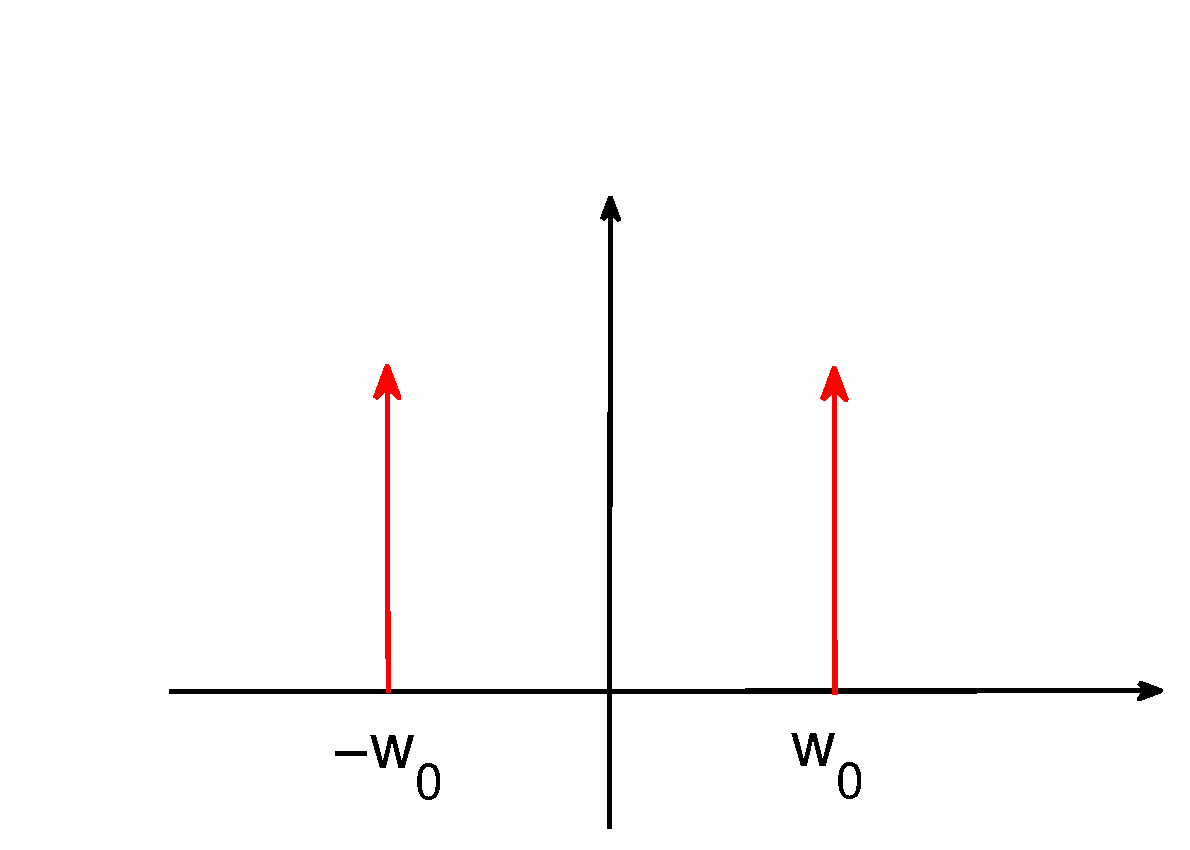
\includegraphics[width=3cm,clip=true,trim=0cm 0cm 0cm 2.5cm]{./Figures/alias1.eps}}\visible<3->{
% 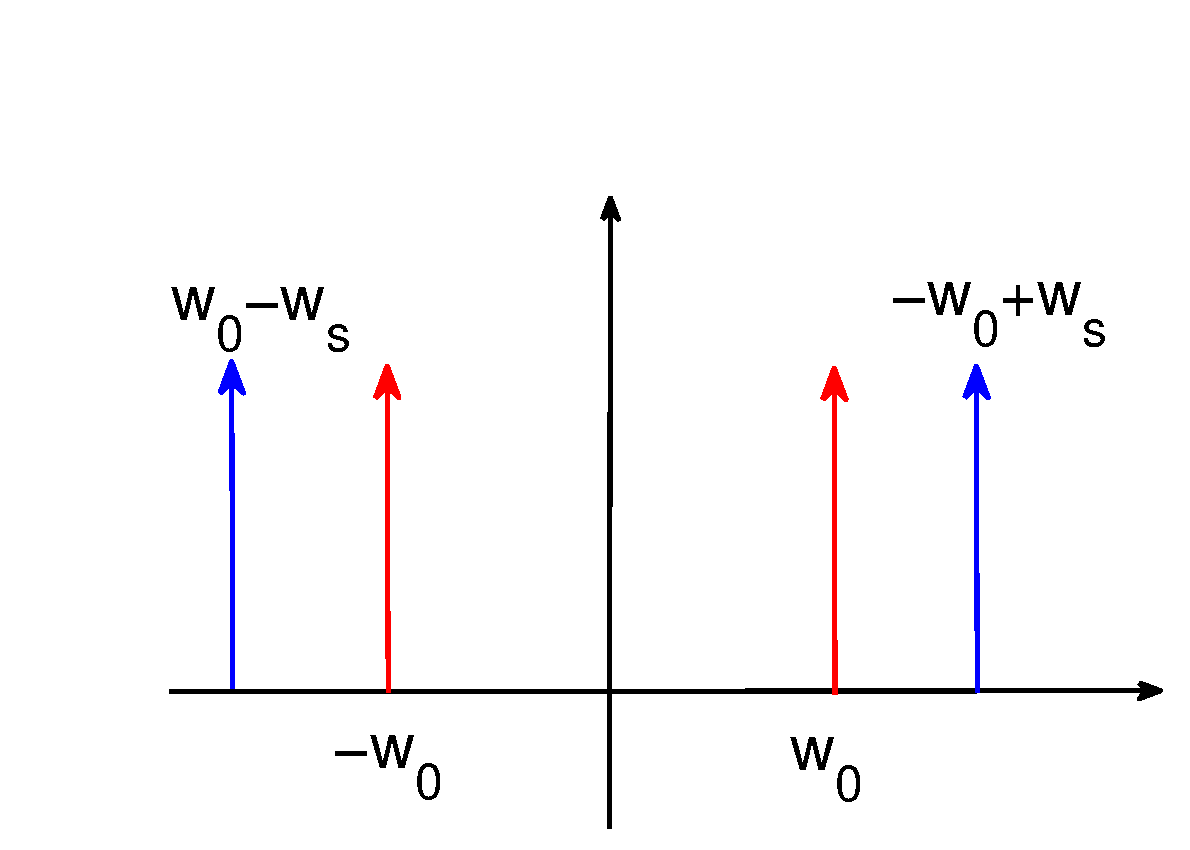
\includegraphics[width=3cm,clip=true,trim=0cm 0cm 0cm 2.5cm]{./Figures/alias2.eps}}
% \end{column}
% \end{columns}

% \vspace{-0.1cm}

% \begin{columns}[c]
% \begin{column}{8.5cm}



% \visible<4->{
% Si $w_s>2w_0$ las únicas componentes espectrales que aparecen dentro del rango de  frecuencias de muestreo son las componentes espectrales de la señal original. }

% \visible<5->{

% \vspace{0.2cm}
% Si $w_s<2w_0$ las componentes espectrales de la señal original no aparecen dentro del rango de frecuencias de muestreo. Las que aparecen son las componentes asociadas a la frecuencia fundamental ($w_0-w_s$ y $-w_0+w_s$). Por lo tanto, se produce el fenómeno de aliasing.}

% \end{column}
% \hspace{-0.5cm}\begin{column}{3cm}

% \visible<4->{
% 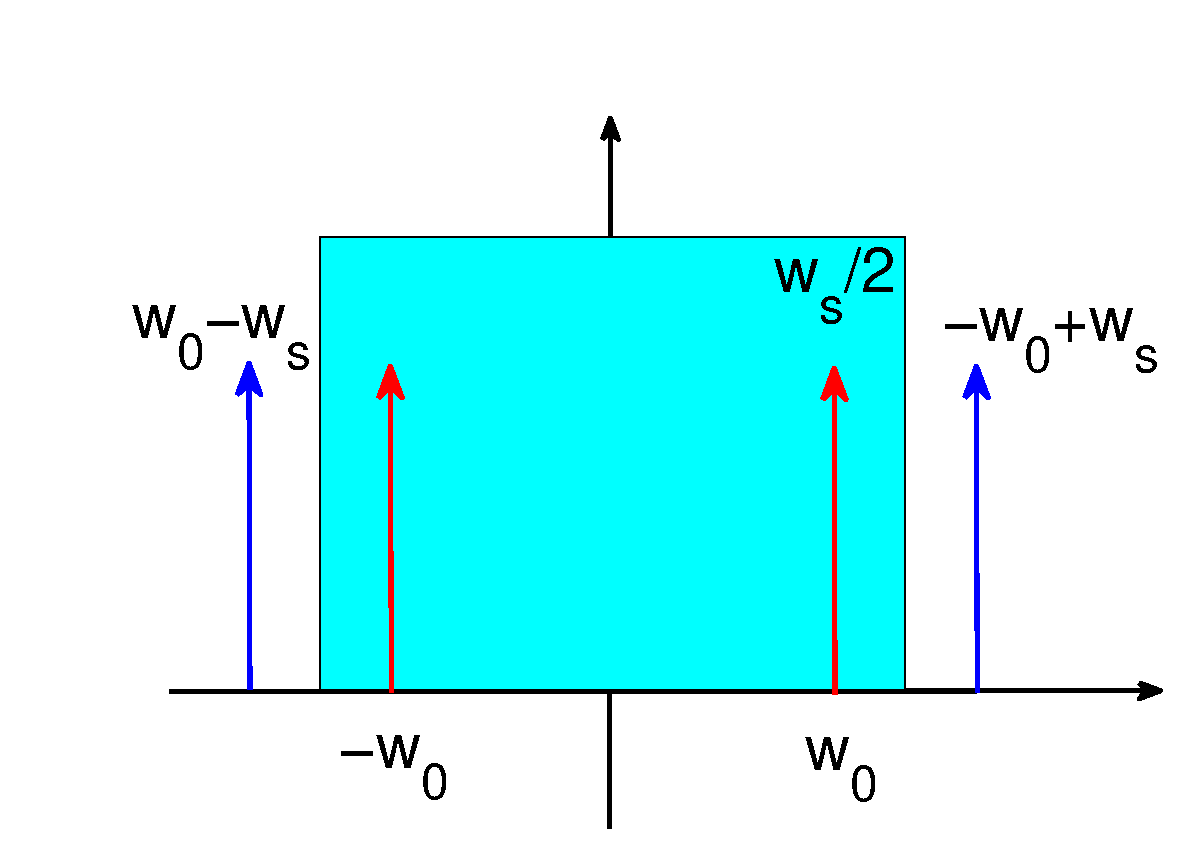
\includegraphics[width=3cm,clip=true,trim=0cm 0cm 0cm 1cm]{./Figures/alias2b.eps}}

% %\vspace{-0.2cm}
% \visible<5->{

% 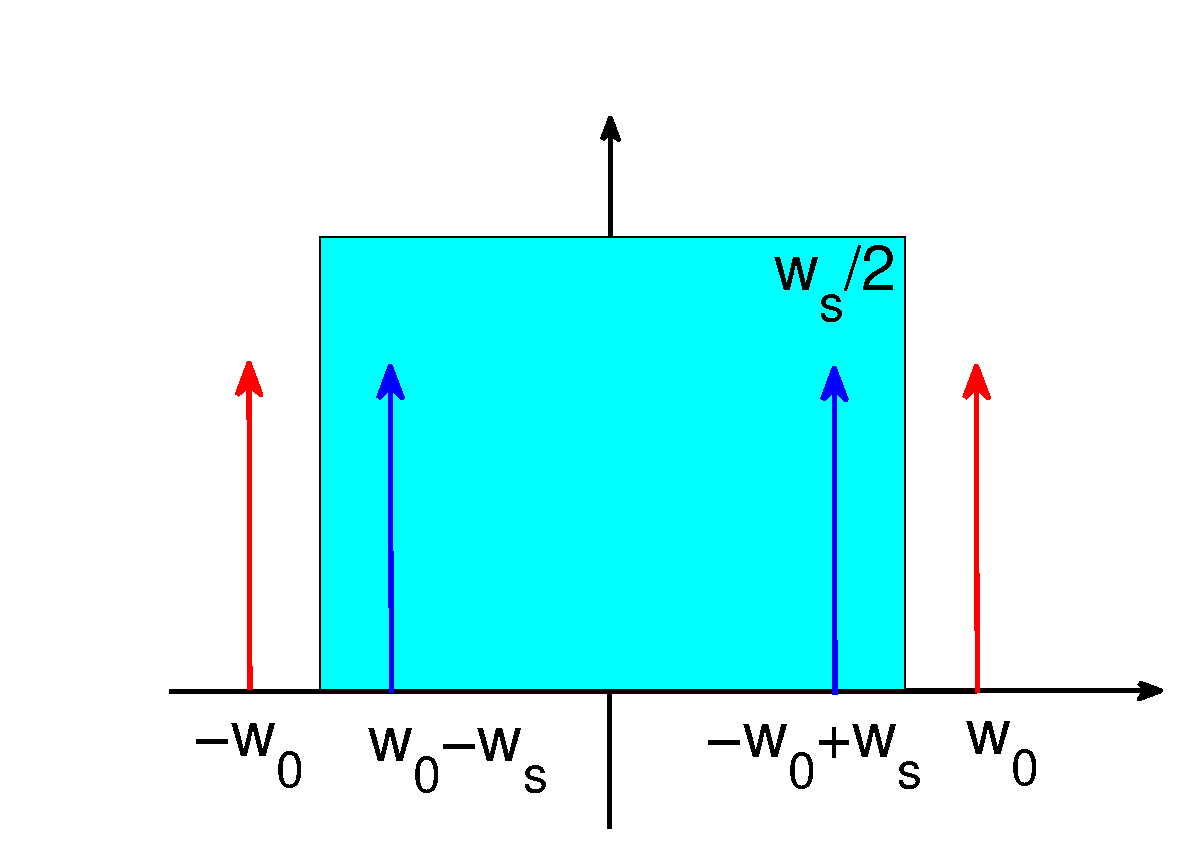
\includegraphics[width=3cm,clip=true,trim=0cm 0cm 0cm 1cm]{./Figures/alias3b.eps}}
% \end{column}
% \end{columns}


% \end{frame}

% %%%%%%%%%%%%%%%%%%%%%%%%%%%%%%%%%%%%%%%%

% \begin{frame}
% \frametitle{Análisis en frecuencia del muestreo natural I}

% \footnotesize

% \begin{itemize}
% \item Muestreo ideal no existe: no se puede tomar una muestra instantáneas.
% \visible<2->{
% \item Habitualmente, lo que se hace es muestrear utilizando un \alert{tren de pulsos}: }

% \begin{itemize}

% \footnotesize

% \vspace{-0.1cm}
% \visible<3->{
% \item Señal discreta: $x_d(n)=x_c(T_sn)$

% \vspace{0.1cm}}

% \visible<4->{
% \item Visión continua de la señal discreta (\alert{muestreo natural, a través del tren de pulsos}):

% \vspace{0.1cm}
% \hspace{0.5cm}	$x_p(t)\!=x_c(t)\!\sum_{k=-\infty}^{\infty} r(t-kT_s)$}

% \vspace{0.1cm}

% \visible<5->{
% \item Transformada de Fourier de $x_p(t)$, propiedad de la multiplicación:

% \vspace{0.1cm}

% \hspace{0.5cm}	$X_p(jw)=\frac{1}{2\pi} (X_c * R)(jw)$

% \vspace{0.1cm}
% }
% \visible<6->{
% \item Transformada de Fourier de $r(t)$, señal periódica de periodo $T_s$:

% \vspace{0.1cm}

% \hspace{0.5cm}	$R(jw)\!\!=\!\!\sum_{k=-\infty}^{\infty} \!\! 2\pi c_k  \delta(w\!-\!kw_s)\!\!=\!\!\sum_{k=-\infty}^{\infty} \!\!\frac{2\pi\tau}{T_s}Sa(w_sk\tau/2) \delta(w\!-\!kw_s)$

% \vspace{0.1cm}

% \hspace{0.5cm}	$c_k=\frac{1}{T_s}\int_{T_s} \Pi_\tau(t) e^{-jkw_st}dt=\frac{1}{T_s}\int_{-\tau/2}^{\tau/2}e^{-jkw_st}dt=$

% \hspace{1cm}$=\frac{1}{T_s}\frac{1}{-jkw_s}(e^{-jw_sk\tau/2}\!-\!e^{jw_sk\tau/2})\!=\!\frac{\tau}{T_s}\frac{sen(w_sk\tau/2)}{w_sk\tau/2}\!=\!\frac{\tau}{T_s}Sa(w_sk\tau/2)$
% }

% \vspace{0.1cm}

% \visible<7->{
% \item Convolución usando deltas:

% \vspace{0.1cm}

% \hspace{1.5cm}	\alert{$X_p(jw)=\frac{\tau}{T_s} \sum_{k=-\infty}^{\infty}Sa(w_sk\tau/2) X_c(j(w-kw_s))$}
% }




% \end{itemize}

% \end{itemize}

% \end{frame}

% %%%%%%%%%%%%%%%%%%%%%%%%%%%%%%%%%%%%%%%%%%%%%%%%

% \begin{frame}
% \frametitle{Análisis en frecuencia del muestreo natural II}



% \vspace{0.1cm}

% Muestreo ideal: \alert{$X_p(jw)=\frac{1}{T_s} \sum_{k=-\infty}^{\infty} X_c(j(w-kw_s))$}

% \vspace{0.1cm}

% Muestreo natural: \alert{$X_p(jw)=\frac{\tau}{T_s} \sum_{k=-\infty}^{\infty}Sa(w_sk\tau/2) X_c(j(w-kw_s))$}

% \vspace{0.4cm}

% \footnotesize

% \begin{columns}[T]
% \begin{column}{6.5cm}

% \hspace{2cm}Muestreo ideal

% \vspace{0.1cm}

% \includegraphics[trim=0cm 0cm 0cm 5cm, clip=true,width=6.5cm]{./Figures/Muestreo2.ps}


% \end{column}
% \begin{column}{6cm}

% \hspace{2cm}Muestreo natural


% \end{column}
% \end{columns}


% \end{frame}
% %%%%%%%%%%%%%%%%%%%%%%%%%%%%%%%%%%%%%%%%

% \subsection{Teorema de Muestreo}

% %%%%%%%%%%%%%%%%%%%%%%%%%%%%%%%%%%%%%%%%


% \begin{frame}
% \frametitle{Teorema de Muestreo}

% \footnotesize

% ¿ Cual es el valor del $T_s$ a partir del cual podemos reconstruir la señal original si tenemos un señal de ancho limitado en frecuencia?

% \vspace{0.2cm}

% \visible<2->{

% \alert{Teorema de Nyquist-Shannon$^1$:}  Para que se pueda reconstruir una se\~{n}al a partir de su muestreo es necesario que la frecuencia de muestreo sea al menos dos veces superior a la mayor frecuencia $w_0$ contenida en la se\~{n}al muestreada: \alert{$w_s=\frac{2\pi}{T_s}>2 w_o$}}

% \vspace{0.2cm}

% \visible<3->{
% \alert{Reformulado con periodos}: $T_s<T_0/2$, con $T_0$ el menor de los periodos de la se\~{n}al original.
% }

% \vspace{0.2cm}

% \visible<4->{
% Es decir, necesitamos muestrear con un periodo que por lo menos sea la mitad del periodo del mas pequeño de la señal original.}

% \vspace{0.2cm}

% \visible<5->{
% \alert{Intuitivamente}:

% \vspace{1cm}

% }


% \visible<2->{
% \rule{10cm}{0.4pt}
% \scriptsize

% $^1$ Nyquist, en 1928, presenta la idea. Shannon, en 1949, lo enuncia como teorema. }


% \end{frame}


% \begin{frame}
% \frametitle{Ejemplos de aliasing de señales sinusoidales III}

% \small

% \hspace{1.9cm}\alert{$x_d(n)=x_c(nT_s)=sen(w_cT_sn+\phi)=sen(w_dn+\phi)$}

% \vspace{-0.1cm}

% \begin{itemize}
% \footnotesize
% \item \color{olivegreen} ¿Se puede muestrear $x_c(t)= sen(\frac{2\pi}{10}t)$ con un periodo de muestreo de 2s? \color{gray}

% \visible<2->{
% \vspace{0.1cm}

% $T=10$. El valor máximo del periodo de muestreo que se puede utilizar es $T_s=\frac{T}{2}=5$.

% \vspace{0.0cm}
% }

% \visible<3->{

% Como estamos muestreando con $2s$ que es menor que $T_s=5$, las muestras que aparecen están relacionadas con la señal original.
% }
% \end{itemize}

% \vspace{-0.5cm}


% \begin{columns}[c]
% \begin{column}{6.8cm}
% \footnotesize

% \begin{itemize}

% \item \color{olivegreen} ¿Se puede muestrear $x_c(t)= sen(\frac{2\pi}{10/6}t)$ con un periodo de muestreo $2s$? \color{gray}

% \visible<4->{
% $T=10/6$. El valor máximo del periodo de muestreo que se puede utilizar es $T_s=\frac{10/6}{2}=5/6$.
% }

% \visible<5->{

% El periodo elegido (2s) es mayor que el límite máximo (5/6s).}\visible<6->{  Por lo tanto, las muestras tienen que estar relacionadas con un alias fundamental (que ya  hemos calculado previamente).
% }
% \end{itemize}
% \end{column}
% \hspace{-0.4cm}\begin{column}{4.5cm}
% {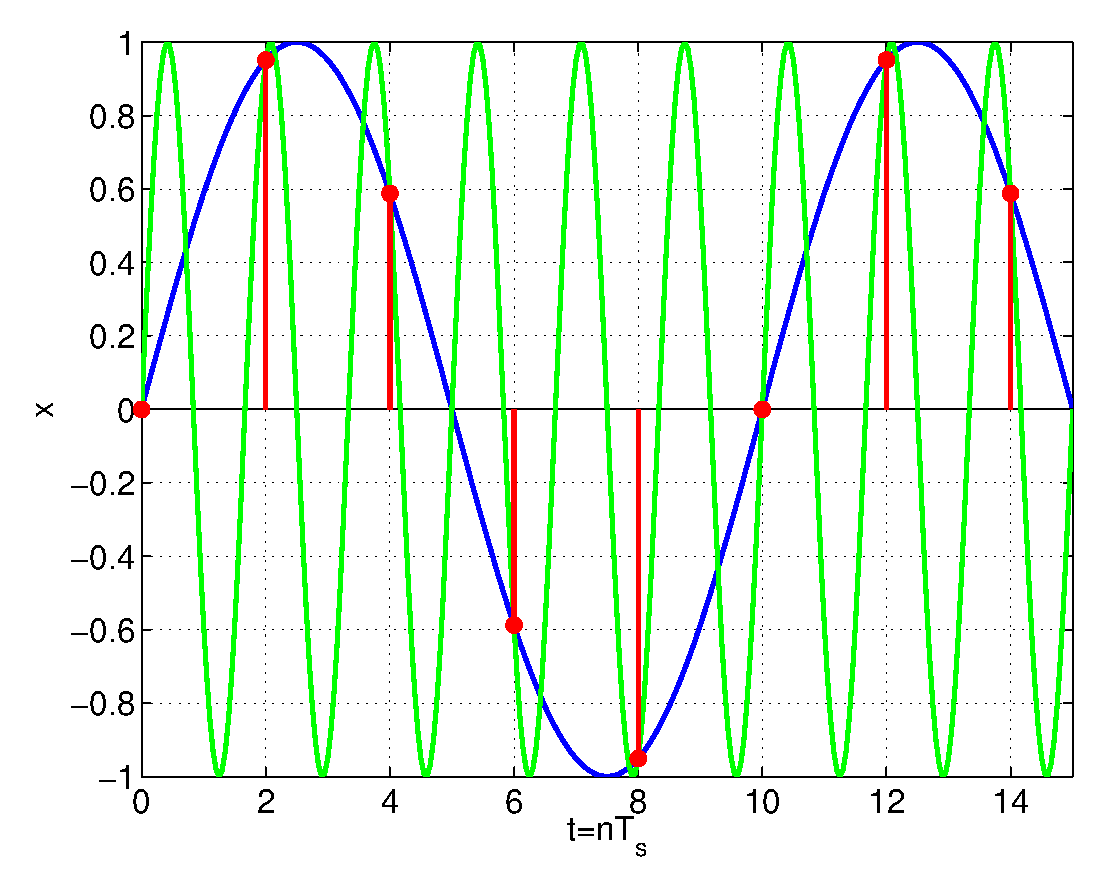
\includegraphics[width=4.5cm]{./Figures/AliasBasic3.eps}}
% \end{column}
% \end{columns}

% \end{frame}

% %%%%%%%%%%%%%%%%%%%%%%%%%%%%%%%%%%%%%%

% \begin{frame}
% \frametitle{Ejemplos de aliasing de señales sinusoidales IV}

% \small

% \hspace{1.9cm}\alert{$x_d(n)=x_c(nT_s)=sen(w_cT_sn+\phi)=sen(w_dn+\phi)$}

% \vspace{-0.1cm}

% \begin{itemize}
% \footnotesize
% \item \color{olivegreen} ¿Se puede muestrear $x(t)=3 sen(\frac{2\pi}{5}t)+ sen(\frac{2\pi}{3}t)$ con un periodo de muestreo de 2s? \color{gray}
% \end{itemize}

% \begin{columns}[c]
% \begin{column}{4.6cm}
% \only<1-4>{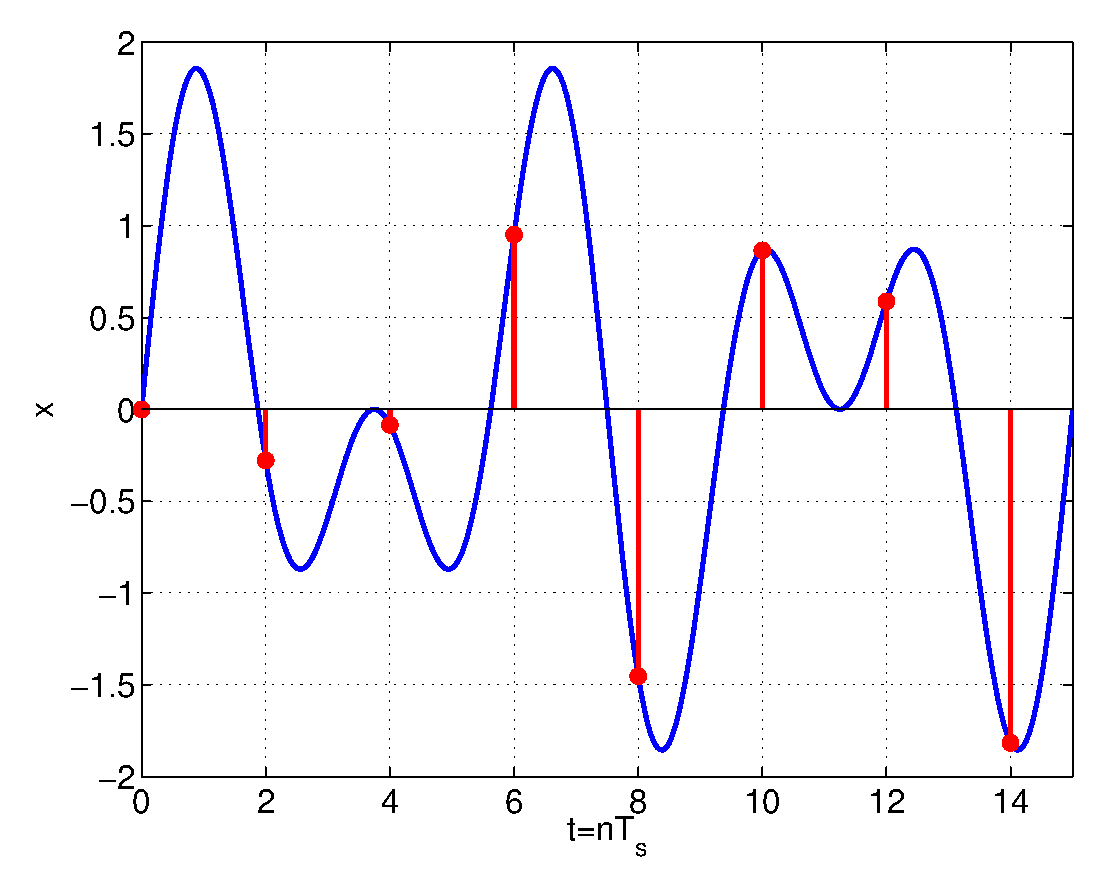
\includegraphics[width=4.5cm]{./Figures/AliasEj3_1.eps}}
% \end{column}
% \begin{column}{6.2cm}

% \color{gray}

% \footnotesize

% $T_1=5$ y $T_2=3$.

% \vspace{0.1cm}
% \visible<2->{
% El periodo máximo con el que se debería muestrear esta señal es: $T_s=\frac{3}{2}=1.5$
% }
% \vspace{0.1cm}
% \visible<3->{
% Muestreamos con una $T_s$ mayor $\rightarrow$ habr\'{a} aliasing (el alias fundamental ya lo hemos calculado previamente). }
% \vspace{0.1cm}
% \end{column}
% \end{columns}

% \vspace{0.2cm}
% \visible<4->{
% \hrule

% \vspace{0.2cm}



% \footnotesize
% \color{gray}
% El teorema de Shannon/Nyquist nos permite saber cuando habr\'{a} aliasing o cuando no. Cuando lo haya, se puede pedir que se calcule el alias fundamental. Cuando no lo haya, idealmente se puede reconstruir la se\~{n}al original continua a partir de las muestras (veremos como m\'{a}s adelante}

% \end{frame}




% \begin{frame}
% \frametitle{Visión Continua y Discreta del Muestreo}

% \footnotesize

% \begin{itemize}
% \item Visión continua (visto en señales de banda limitada, muestreo ideal):

% \begin{itemize}

% \vspace{-0.1cm}

% \footnotesize
% \item Señal continua $x_c(t)$ banda limitada: $X_c(jw)=0$ para $|w|>w_M$

% \vspace{0.1cm}

% \item Visión continua de la señal discreta: $x_p(t)\!=\!\sum_{k=-\infty}^\infty x_c(t)\delta(t\!-\!kT_s)$

% \vspace{0.1cm}
% \item CTFT señal muestreada ($w_s=\frac{2\pi}{T_s}$):

% \vspace{-0.1cm}

% \begin{itemize}
% \item Propiedad del producto: $X_p(jw)\!\!=\!\!\frac{1}{T_s}\!\! \sum_{k=-\infty}^{\infty}\!X_c(j(w\!-\!kw_s))$

% \vspace{0.1cm}

% \visible<4->{\item Definición: $X_p(jw)=\sum_{k=-\infty}^\infty x_c(kTs)e^{-jwkT_s}$}
% \end{itemize}

% \end{itemize}

% \item Visión discreta de la señal muestreada:

% \begin{itemize}

% \vspace{-0.1cm}

% \footnotesize
% \item Señal muestreada: $x_d(n)=x_c(nT_s)$

% \vspace{0.1cm}

% \visible<2->{\item DTFT señal muestreada ($\Omega$ para distinguirla de la $w$ continua):}

% \begin{itemize}

% \visible<3->{\item Definición: $X_d(e^{j\Omega})=\sum_{n=-\infty}^\infty x_c(nTs)e^{-j\Omega n}$}

% \vspace{0.1cm}

% \visible<5->{\item Comparándo $X_d(e^{j\Omega})$ con $X_p(jw)$, coinciden si $\Omega=\omega T_s $}

% \vspace{0.1cm}

% \visible<6->{\item Sustituyendo $w$ por $\frac{\Omega}{T_s}$ en $X_c(jw)$, se obtiene que:

% \vspace{0.1cm}

% $X_d(e^{j\Omega})\!\!=\!\!\frac{1}{T_s}\!\! \sum_{k=-\infty}^{\infty}\!X_c(j(\frac{\Omega}{T_s}\!-\!kw_s))=\!\!\frac{1}{T_s}\!\! \sum_{k=-\infty}^{\infty}\!X_c(j(\frac{\Omega-2k\pi}{T_s}))$}


% \end{itemize}


% \end{itemize}





% \end{itemize}

% \end{frame}

% \begin{frame}
% \frametitle{Visión Continua y Discreta del Muestreo}

% \footnotesize

% \vspace{0.3cm}

% \begin{columns}[T]
% \begin{column}{6.5cm}

% \centering
%     Visión Continua


% $X_p(jw)\!\!=\!\!\frac{1}{T_s}\!\! \sum_{k=-\infty}^{\infty}\!X_c(j(w\!-\!kw_s))$


% \vspace{0.2cm}

% \includegraphics[trim=0cm 0cm 0cm 5cm, clip=true,width=6.5cm]{./Figures/Muestreo2.ps}


% \end{column}
% \begin{column}{6cm}

% \centering

% \vspace{0.1cm}

%   Visión Continua y Discreta


%   ($\Omega=wT_s$)


%   $X_d(e^{j\Omega})=\frac{1}{T_s}\!\! \sum_{k=-\infty}^{\infty}\!X_c(j(\frac{\Omega-2k\pi}{T_s}))$

% \vspace{0.2cm}

% \includegraphics[trim=0cm 0cm 0cm 1cm, clip=true,width=4cm]{./Figures/MuestreoContinuoDiscreto.ps}
% \end{column}
% \end{columns}


% \end{frame}

\section{Reconstrucción continua de señales muestreadas}

\subsection{Reconstrucción ideal}

\begin{frame}
\frametitle{Reconstrucción ideal I}

\vspace{-0.2cm}

\footnotesize
\begin{itemize}
\item Señal banda limitada: \alert{$X_c(jw)=0$ para $|w|>w_M$}

\item Señal muestreada idealmente: \alert{$x_p(t)\!=\!x_c(t)\!\cdot \! \sum_{k=-\infty}^{\infty}\! \!\delta(t-kT_s)$}

\item CTFT señal muestreada idealmente: \alert{$X_p(jw)\!\!=\!\!\frac{1}{T_s}\!\! \sum_{k=-\infty}^{\infty}\!X_c(j(w\!-\!kw_s))$}
\end{itemize}



\hspace{1.0cm}\alert{¿Reconstrucción de la señal original a partir de la muestreada?}


\vspace{-0.3cm}

\footnotesize
\begin{columns}[c]
\begin{column}{4.5cm}
\visible<2->{\includegraphics[width=4.5cm]{./Figures/RecIdeal.ps}}
\end{column}
\begin{column}{7cm}
\begin{itemize}

\visible<3->{
\item Respuesta en dominio frecuencia:

$Y(jw)=H(jw)\cdot X_p(jw)$}

\visible<4->{
\item Filtro paso bajo ideal:

$H(jw)=T_s \Pi (\frac{w}{2w_c})$ 

\hspace{0.3cm} con $w_M\!<\!w_c\!<\!w_s\!-\!w_M$

$Y(jw)=H(jw)\cdot X_p(jw)=X_c(jw)$}


\visible<5->{
\item Respuesta en dominio temporal:

$y(t)=(h*x_p)(t)$}

\visible<6->{
\item Función Ponderatriz del Filtro:

$Sa(\frac{t}{2}) \rightarrow 2 \pi \Pi(w)$

$Sa(\frac{2w_ct}{2}) \rightarrow \frac{2 \pi}{2w_c} \Pi(\frac{w}{2w_c}) \rightarrow \frac{\pi}{w_c} \Pi(\frac{w}{2w_c}) $

$h(t)=\frac{T_s w_c}{\pi}Sa(w_ct)$
}


\end{itemize}
\end{column}

\end{columns}


\end{frame}

%%%%%%%%%%%%%%%%%

\begin{frame}
\frametitle{Reconstrucción ideal II}

\footnotesize

\begin{itemize}

\color{gray}

\item Señal original  $x_c(t)$ de banda limitada ($X_c(w)=0$ para $|w|>w_m$)

\item Señal muestreada idealmente: $x_p(t)\!=\!x_c(t)\!\cdot \! \sum_{k=-\infty}^{\infty}\! \!\delta(t-kT_s)$

\item Función ponderatriz del filtro: $h(t)=\frac{T_s w_c}{\pi}Sa(w_ct)$


\item Salida del filtro: $y(t)=(h*x_p)(t)$

\color{black}

\vspace{0.1cm}
\visible<2->{
$x_p(t)\!=\! \sum_{k=-\infty}^{\infty} x_c(kT_s) \delta(t-kT_s)$}

\visible<3->{
\vspace{0.1cm}

\alert{$y(t)=x_c(t)=\! \sum_{k=-\infty}^{\infty} x_c(kT_s) \frac{T_s w_c}{\pi}Sa(w_c(t-kT_s))\:\:\:$}   con $w_M\!<\!w_c\!<\!w_s\!-\!w_M$
}
\scriptsize

\visible<4->{
\item Se reconstruye la señal original combinando un número infinito de funciones de muestreo desplazadas un múltiple entero del periodo de muestreo y ponderadas con un factor que incluye el valor de la señal original en cada instante.

\item La función interpola los valores de la señal muestreada en todo instante $k\!\in\!(-\infty,\!\infty)$ con funciones de muestreo desplazadas múltiplos del periodo de muestreo.

\item La interpolación con infinitos términos no es computacionalmente eficiente. Y la señales limitadas en el tiempo (cuya muestra tiene un número finito de términos) no son de banda limitada. Sin embargo, si la señal se atenúa suficientemente en frecuencia, se podría reconstruir una señal bastante próxima a la original.

\item La alternativa de construir el filtro ideal ($h(t)=\frac{T_s w_c}{\pi}Sa(w_ct)$) y pasar la señal muestreada idealmente a través de él no es factible. Ya que el filtro ideal no es causal (presenta una señal no nula a la $\delta(t)$ para $t<0$).
}

\end{itemize}

\end{frame}

\begin{frame}
\frametitle{Ejemplo de Reconstrucción ideal}




\scriptsize
 Señal original  $x_c(t)$ de banda limitada ($X_c(w)=0$ para $|w|>w_M$)

Señal muestreada $x(n)=x(nT_s)$ con $w_s=\frac{2\pi}{T_s}$ y $w_s>2w_M$.
 
 Señal reconstruida $y(t)\!=\!\! \sum_{k=-\infty}^{\infty} \!x_c(kT_s) \frac{T_s w_c}{\pi}Sa(w_c(t\!-\!kT_s))$  con $w_M\!\!<\!\!w_c\!\!<\!\!w_s\!-\!w_M$

\vspace{-0.05cm}

\rule{11cm}{0.4pt}



\footnotesize
\color{olivegreen}Ejemplo: Reconstruir la señal $x(t)=sen(w_0 t)$ a partir de sus muestras $x(n)=sen(w_0 T_s n)$, con $w_0=\frac{2\pi}{10}$ y $T_s=4$.

\visible<2->{\vspace{0.1cm}
\color{gray}

$w_M=w_0=\frac{2\pi}{10}$}


\vspace{0.1cm}

\visible<3->{

$w_s=\frac{2\pi}{T_s}=\frac{2\pi}{4}>2\frac{2\pi}{10}$. Por lo tanto, se puede reconstruir la señal original con un filtro paso baja ideal con $\frac{2\pi}{10}<w_c<\frac{6\pi}{20}$
}



\visible<4->{
 \hspace{1.5cm}	$w_c=\frac{w_s}{2}=\frac{2\pi}{8}$                                 \hspace{4.3cm}	$w_c=\frac{2\pi}{7}$}

\color{black}




\begin{columns}[c]
\begin{column}{5cm}
\only<4|handout:0>{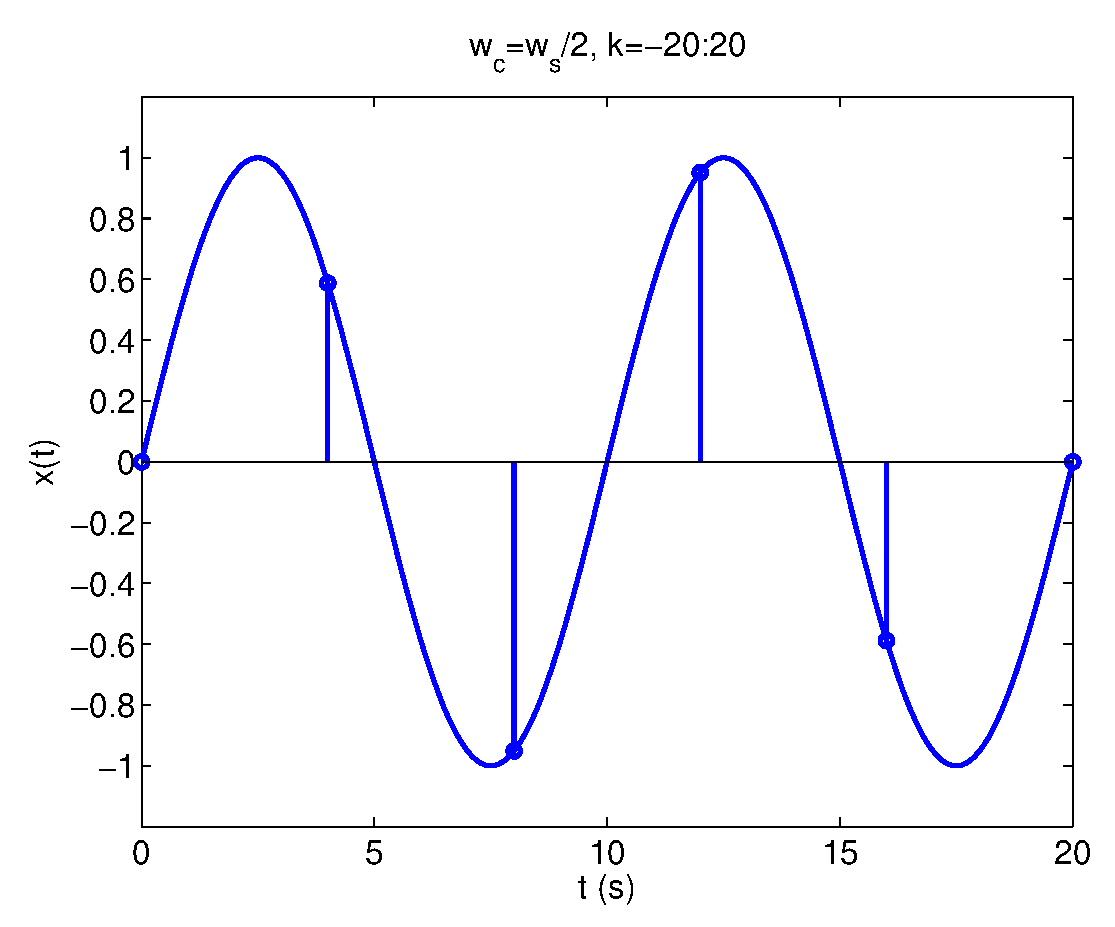
\includegraphics[width=4.3cm]{./Figures/RecIdealEjem1_1.eps}}\only<5|handout:0>{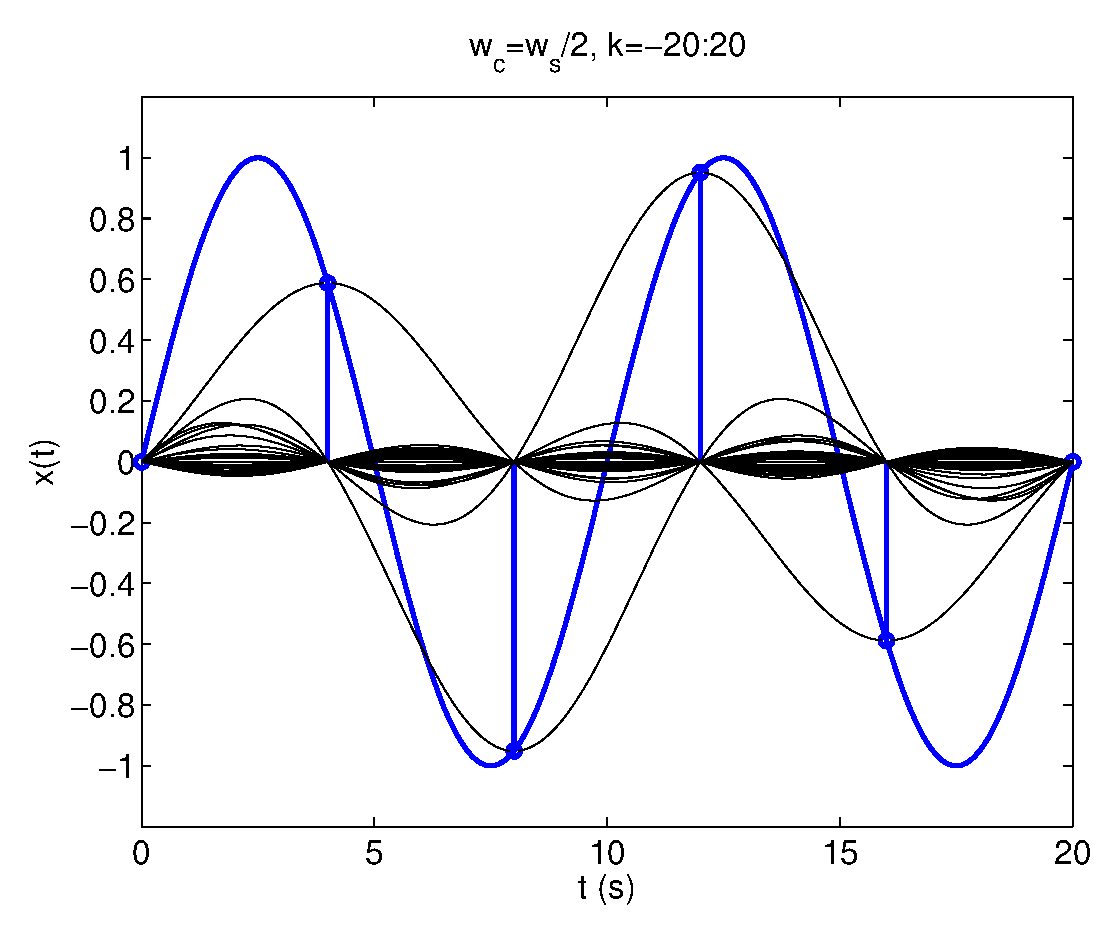
\includegraphics[width=4.3cm]{./Figures/RecIdealEjem1_2.eps}}\only<6->{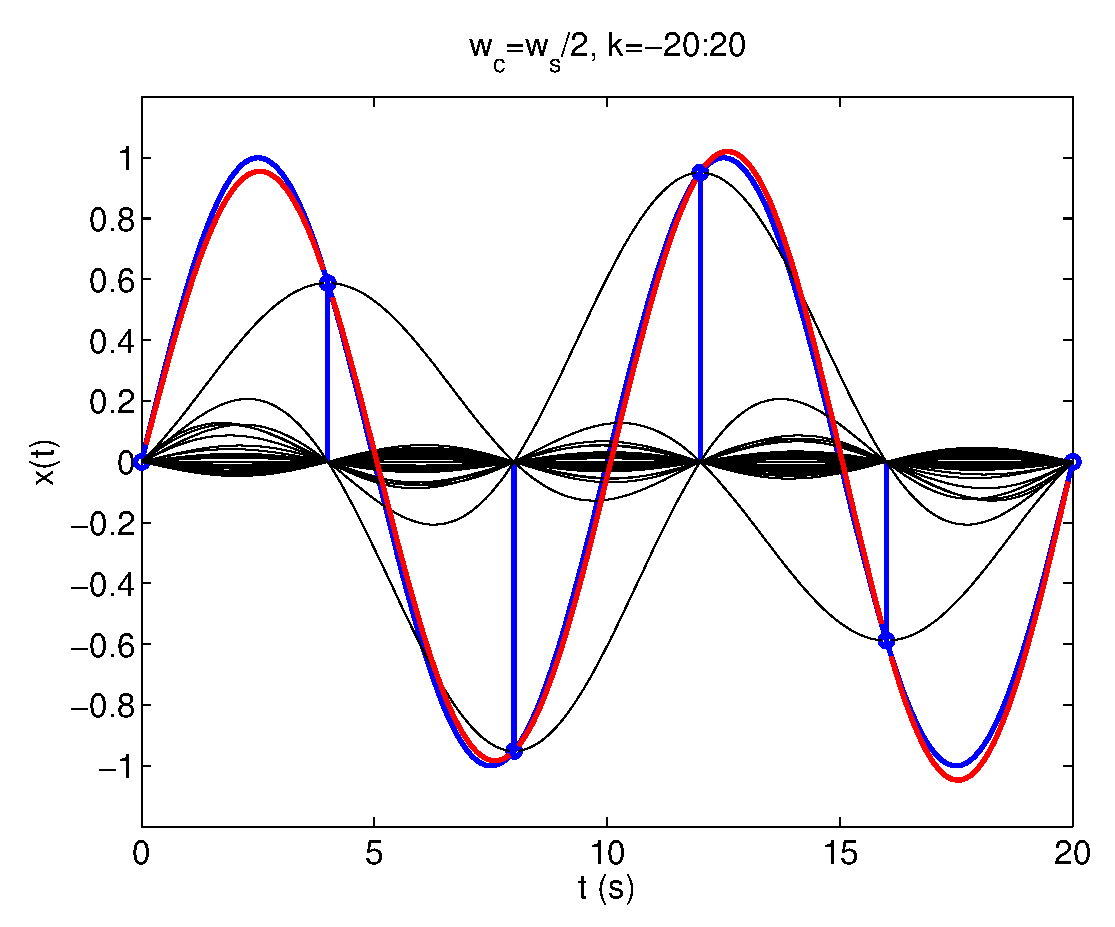
\includegraphics[width=4.3cm]{./Figures/RecIdealEjem1_3.eps}}
\end{column}
\begin{column}{5cm}
\only<7|handout:0>{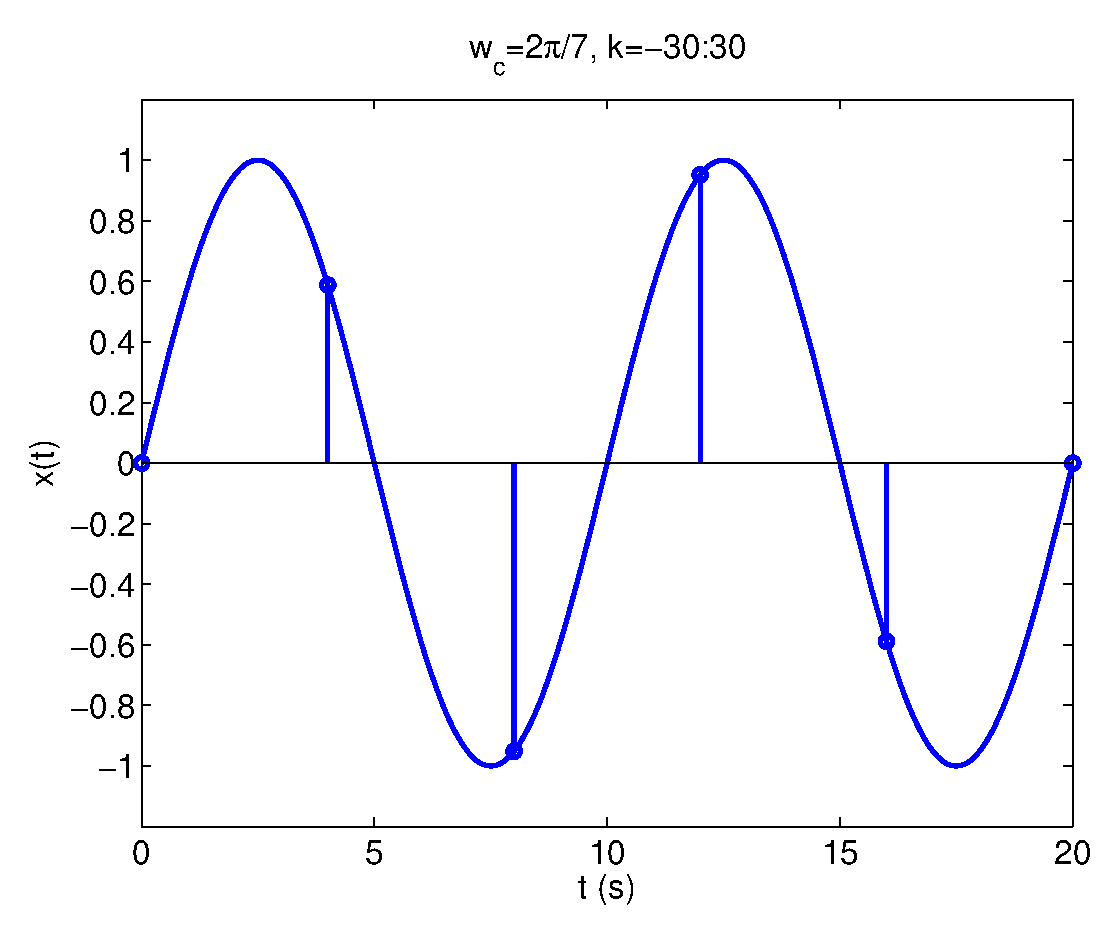
\includegraphics[width=4.3cm]{./Figures/RecIdealEjem2_1.eps}}\only<8|handout:0>{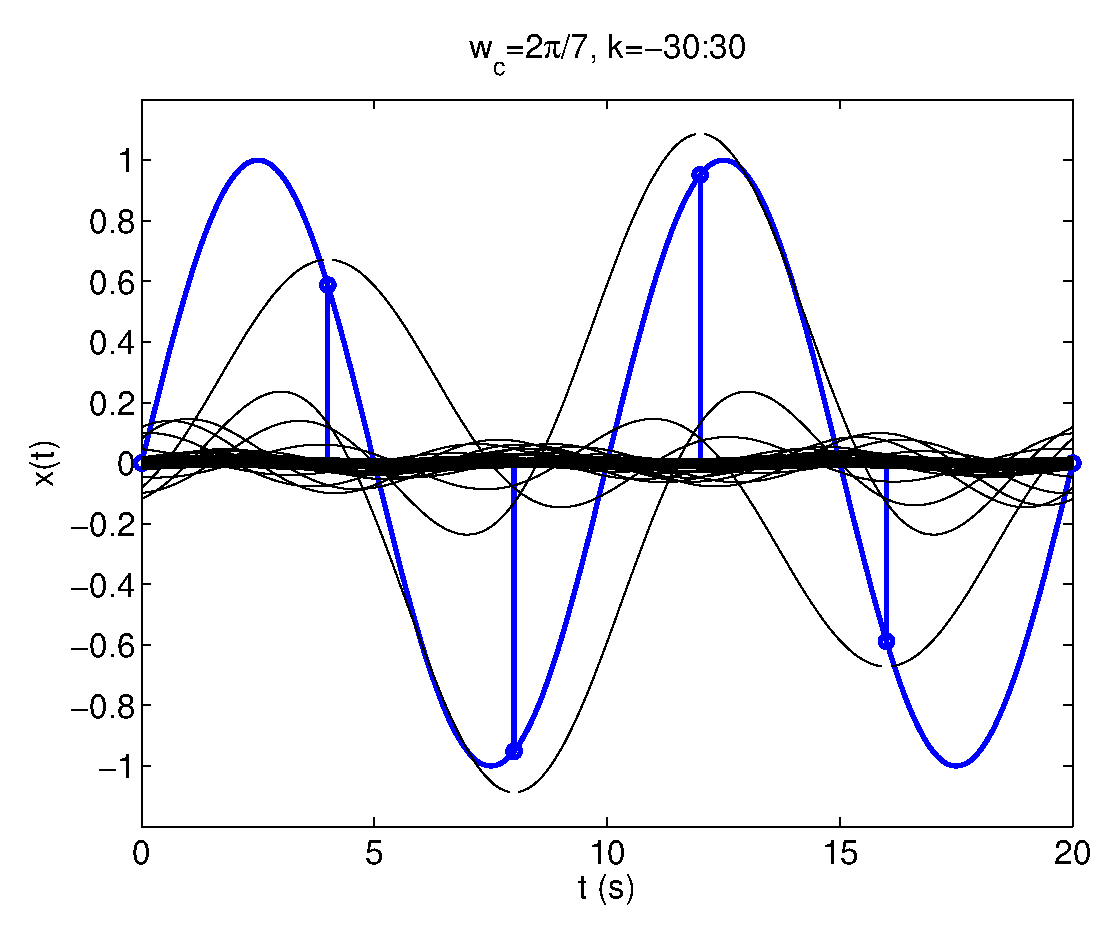
\includegraphics[width=4.3cm]{./Figures/RecIdealEjem2_2.eps}}\visible<9->{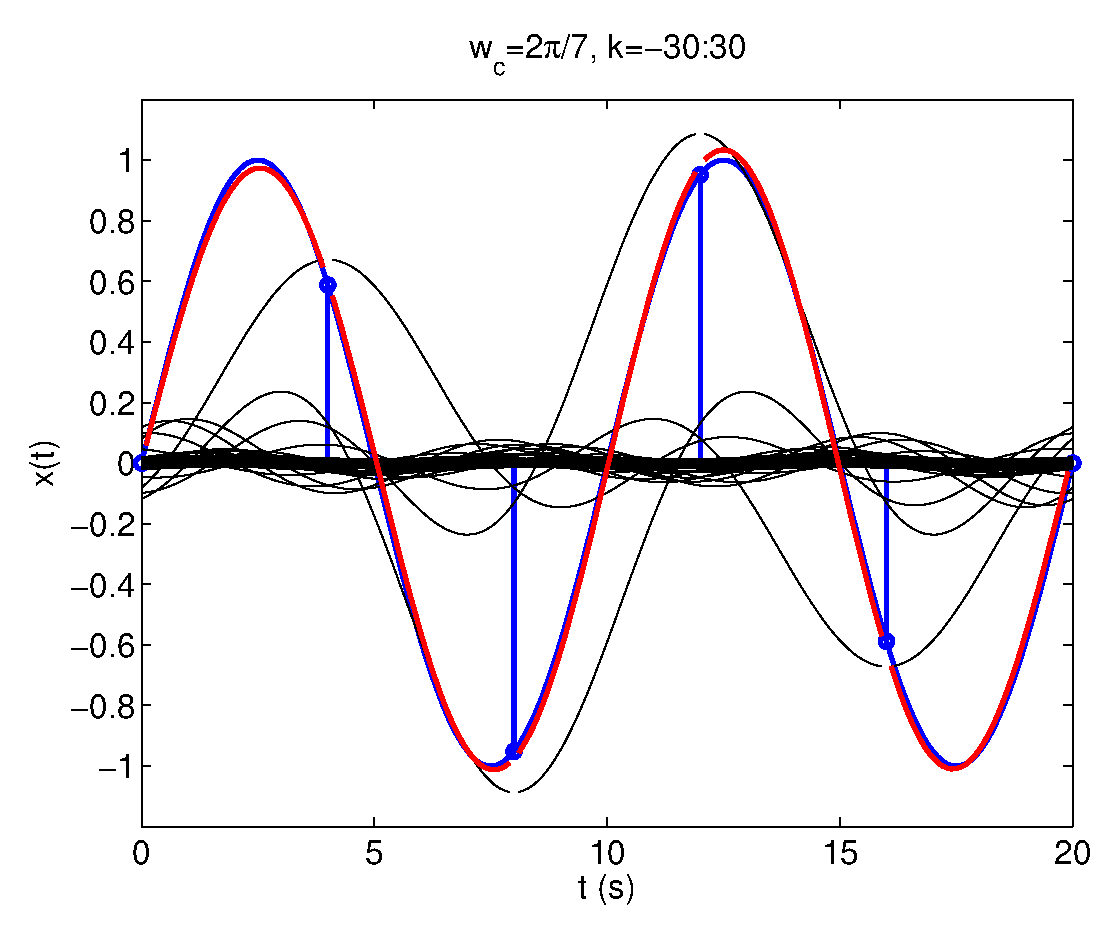
\includegraphics[width=4.3cm]{./Figures/RecIdealEjem2_3.eps}}
\end{column}
\end{columns}

\end{frame}

\subsection{Reconstrucción mediante interpolación}

\begin{frame}
\frametitle{Reconstrucción mediante interpolación I}

\footnotesize 
\begin{itemize}
\item Aunque la reconstrucción a través de un filtro paso baja ideal se puede considerar un método de interpolación de las infinitas muestras de la señal, ésta no se puede realizar de forma computacionalmente eficiente.
\item Por lo tanto, se utilizan métodos alternativos, más sencillos en los que únicamente se interpolan un número finito de muestras:
\begin{itemize}
\footnotesize 
\item Retenedor de orden cero (zero-order holder, ZOH): mantiene constante el valor de la muestra hasta el instante siguiente.
\item Retenedor de orden uno (first-order holder, FOH): interpola lineamente entre dos muestras sucesivas.
\item Retenedor de orden dos (second-order holder, SOH): interpola cuadraticamente entre tres muestras sucesivas.

\end{itemize}

\item Ninguno de estos interpoladores permiten reconstruir totalmente la señal, ya que modifican el espectro en frecuencia de la señal muestreada que los atraviesa. Para verlos los cambios en frecuencia de la señal, podemos analizar el espectro de los retenedores.

\end{itemize}
\end{frame}

\begin{frame}
\frametitle{Reconstrucción mediante interpolación II}

\footnotesize

\vspace{-0.1cm}

\hspace{1.0cm}{$x_p(t)\!= \! \sum_{k=-\infty}^{\infty}x_c(t)\delta(t-kT_s)$}  \hspace{0.3cm} y \hspace{0.3cm} {$X_p(jw)\!\!=\!\!\frac{1}{T_s}\!\! \sum_{k=-\infty}^{\infty}\!X_c(j(w\!-\!kw_s))$}

\rule{11cm}{0.4pt}

\begin{columns}[c]
\begin{column}{4.5cm}
\footnotesize

\vspace{-0.9cm}

\begin{itemize}
\item Retenedor de orden cero:
\end{itemize}

 \begin{figure}
  \centering
  \small
\scalebox{0.8}{
  \begin{psmatrix}[mnode=r,colsep=0.5,rowsep=0.3]
  [name=inc1] &&& &[name=continuo]  \visible<1-> {\psframebox[fillstyle=solid,fillcolor=yellow,framesep=2pt,linecolor=gray,linewidth=0.4pt]{\parbox[c]{8ex}{\centering ZOH}}} & &&&  [name=ind2]\\
     \visible<1->{\ncline[linecolor=black]{->}{inc1}{continuo}  \Bput{$\delta(t)$}\Aput{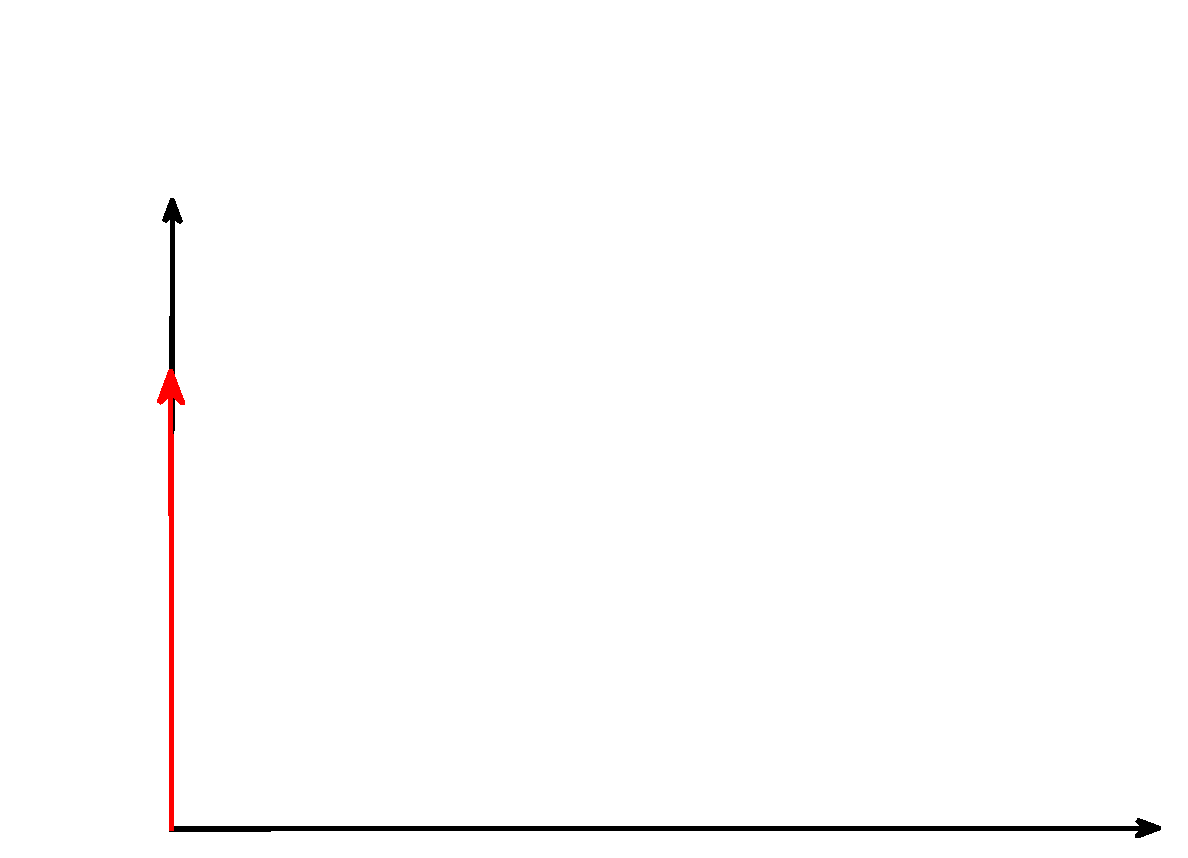
\includegraphics[width=1.5cm]{./Figures/inputimp.eps} }}
   \visible<1->{\ncline[linecolor=black]{->}{continuo}{ind2}  \Bput{h(t)}\Aput{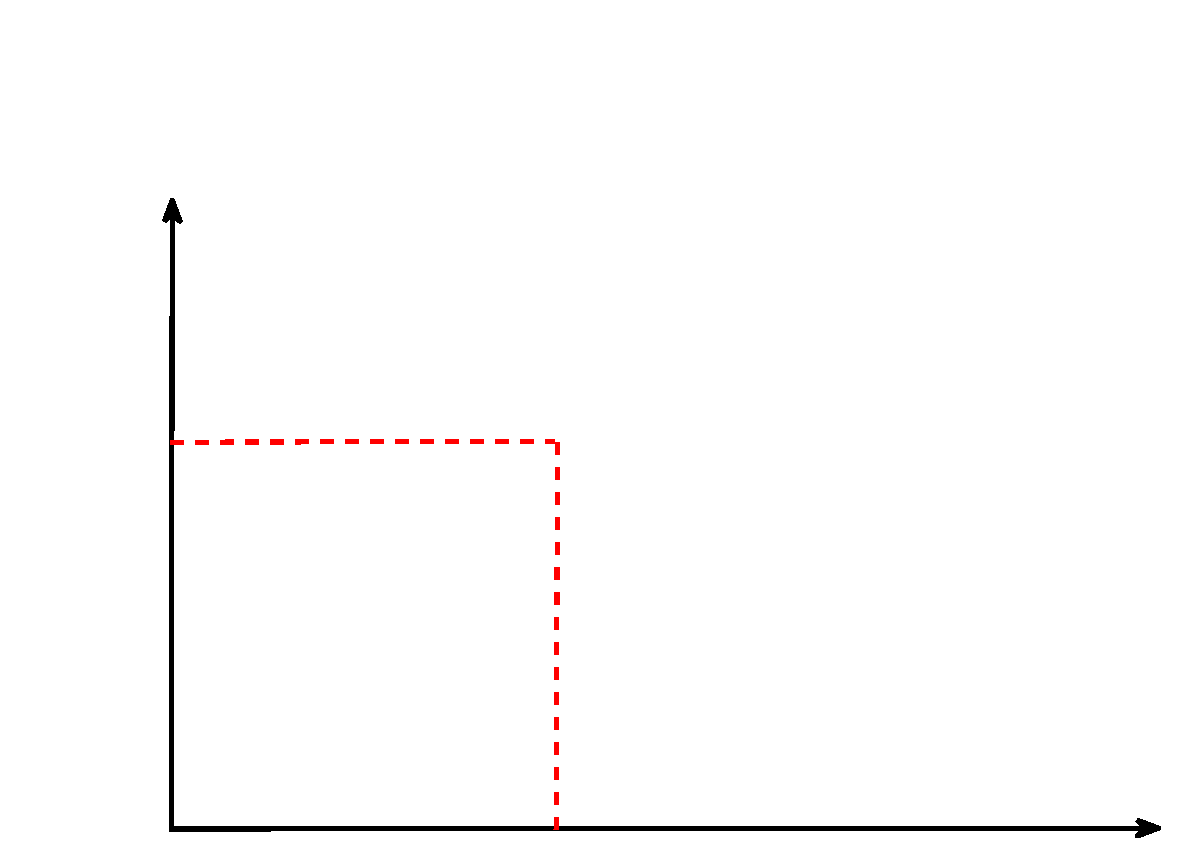
\includegraphics[width=1.5cm]{./Figures/outputimp.eps} }}
%\visible<1->{\ncline[linecolor=black]{-}{ind1}{jjj} }
    \end{psmatrix}  
  }
\end{figure}

\vspace{-0.4cm}
\visible<2->{
\begin{itemize}
\item Retenedor de orden uno:
\end{itemize}

 \begin{figure}
  \centering
  \small
\scalebox{0.8}{
  \begin{psmatrix}[mnode=r,colsep=0.5,rowsep=0.3]
  [name=inc1] &&& &[name=continuo]  \visible<1-> {\psframebox[fillstyle=solid,fillcolor=yellow,framesep=2pt,linecolor=gray,linewidth=0.4pt]{\parbox[c]{8ex}{\centering FOH}}} & &&&  [name=ind2]\\
     \visible<1->{\ncline[linecolor=black]{->}{inc1}{continuo}  \Bput{$\delta(t)$}\Aput{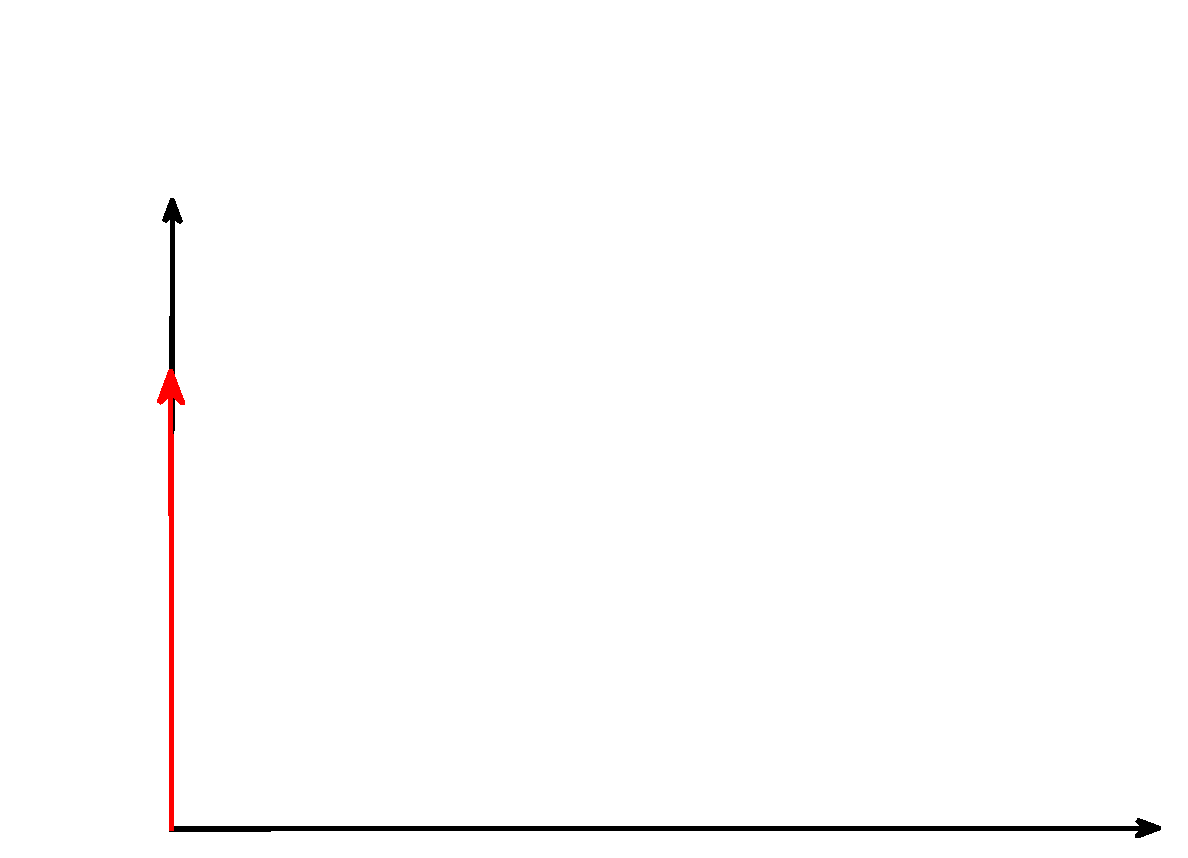
\includegraphics[width=1.5cm]{./Figures/inputimp.eps} }}
   \visible<1->{\ncline[linecolor=black]{->}{continuo}{ind2}  \Bput{h(t)}\Aput{}}
%\visible<1->{\ncline[linecolor=black]{-}{ind1}{jjj} }
    \end{psmatrix}  
  }
\end{figure}

\vspace{-0.5cm}
}
\visible<3->{
\begin{itemize}
\item Filtro paso bajo ideal:

(con $w_c=\frac{w_s}{2}$)
\end{itemize}
}

\end{column}
\begin{column}{6cm}

$h(t)=\Pi(\frac{t-T_s/2}{T_s})$  

\vspace{0.1cm}

$y(t)=(h*x_p)(t)=$

\vspace{0.1cm}

\hspace{0.7cm}$=\sum_{k=-\infty}^{\infty}x_c(kT) \Pi(\frac{t-T_s/2-kT_s}{T_s})$

\vspace{0.1cm}

$H(jw)=e^{jw\frac{T_s}{2}} T_s Sa(T_s w/2)$

\vspace{0.1cm}

\rule{5cm}{0.4pt}

\visible<2->{
$h(t)=\Lambda(\frac{t}{T_s})$  

\vspace{0.1cm}

$y(t)=(h*x_p)(t)=$

\vspace{0.1cm}

\hspace{0.7cm}$=\sum_{k=-\infty}^{\infty}x_c(kT) \Lambda(\frac{t-kT_s}{T_s})$

\vspace{0.1cm}

$H(jw)=T_s Sa^2(T_s w/2)$

\vspace{0.1cm}

%%%%%%%%%%%%%%%%%%%%
%%%%%%%%%%%%%%%%%%%%
\rule{5cm}{0.4pt}}

\visible<3->{
\vspace{0.1cm}

\footnotesize

$h(t)=Sa(\frac{w_s t}{2})$

\vspace{0.1cm}

$y(t)\!=\!\! \sum_{k=-\infty}^{\infty} \!x_c(kT_s) Sa(\frac{w_s(t\!-\!kT_s)}{2})$ 

\vspace{0.1cm}

$H(jw)=T_s \Pi(\frac{w}{w_s})$

\vspace{0.0cm}
}



\end{column}
\end{columns}



\end{frame}

\begin{frame}
\frametitle{Reconstrucción mediante interpolación III}


\begin{columns}[c]
\begin{column}{5cm}
\includegraphics[width=5cm]{./Figures/RecIdeal.ps}
\end{column}
\begin{column}{7cm}
\begin{itemize}
\footnotesize
\item Retenedor orden cero:
$H(jw)=e^{jw\frac{T_s}{2}} T_s Sa(T_s w/2)$

\item Retenedor orden uno:
$H(jw)=T_s Sa^2(T_s w/2)$

\item Filtro ideal:

$H(jw)=T_s \Pi(\frac{w}{w_s})$
\end{itemize}

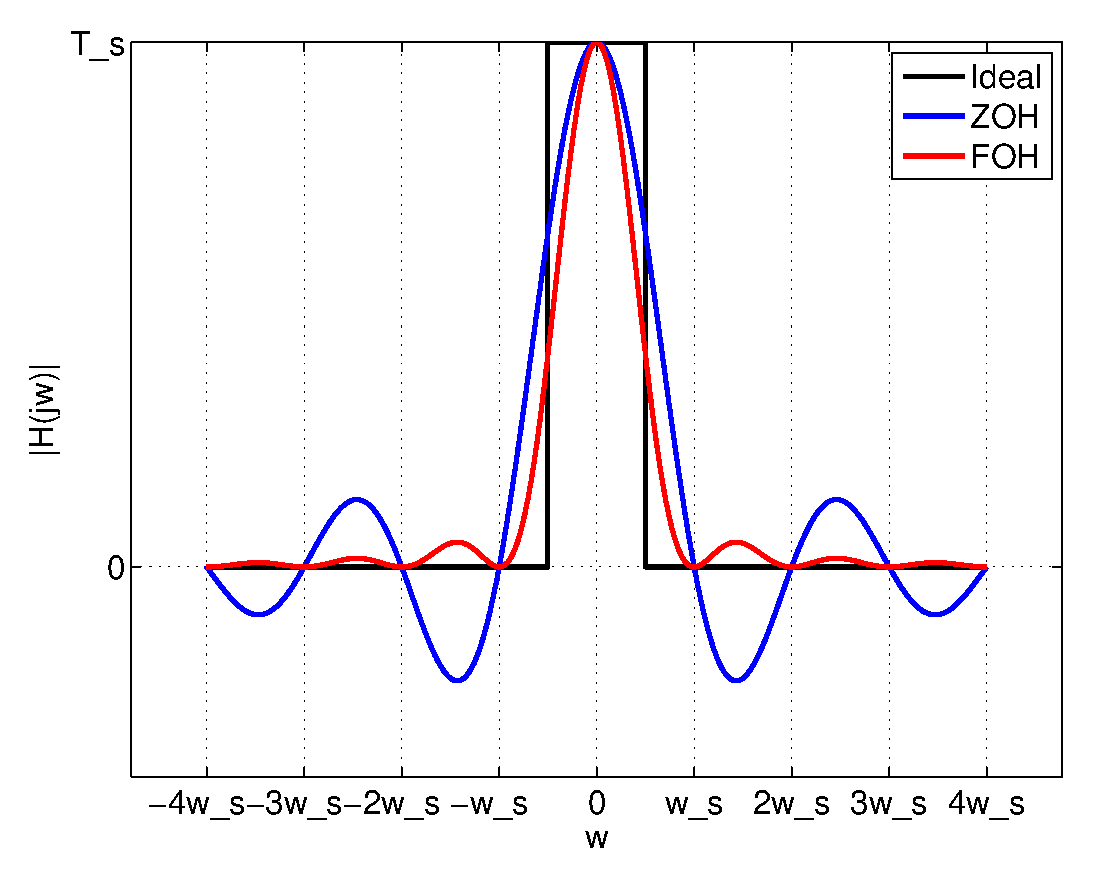
\includegraphics[width=4.5cm]{./Figures/Interpolacion.eps}

\end{column}
\end{columns}


\end{frame}


\begin{frame}
\frametitle{Retenedor de orden uno (FOH)}

\footnotesize

\begin{columns}[c]
\hspace{-0.6cm}\begin{column}{8cm}
\begin{itemize}
\item Versión no causal : 
\begin{itemize}

\footnotesize

\item $h(t)=\Lambda(\frac{t}{T_s})$

\item $y(t)=\sum_{k=-\infty}^\infty x_c(kT)\Lambda(\frac{t-kT_s}{T_s})$

\visible<3->{

\vspace{0.1cm}

\item Es no causal porque:

\begin{itemize}

\item Durante el periodo $t \in (kT_s,(k\!+\!1)T_s)$:  $y(t)=x_c(kT)+\frac{x_c((k+1)T)-x_c(kT)}{T_s} (t-kT_s)$. Depende de un valor fúturo. 

\item Su h(t) toma valores no nulos en instantes previos a t=0.

\end{itemize}
}

\end{itemize}

\visible<4->{

\item Versión causal: }

\begin{itemize}
\footnotesize
\visible<4->{\item Durante el periodo $t \in (kT_s,(k\!+\!1)T_s)$: $y(t)=x_c(kT)+\frac{x_c(kT)-x_c((k-1)T)}{T_s} (t-kT_s)$}

\vspace{0.1cm}

\visible<6->{
\item $h(t)=\Pi(\frac{t-T_s/2}{T_s})(1+\frac{t}{T_s})-\Pi(\frac{t-3T_s/2}{T_s})\frac{t-T_s}{T_s}$}

\vspace{0.1cm}
\visible<7->{
\item Se puede calcular el espectro del filtro (Matlab)}
\end{itemize}


\end{itemize}
\end{column}
\hspace{-0.6cm}\begin{column}{4cm}
\only<1|handout:0>{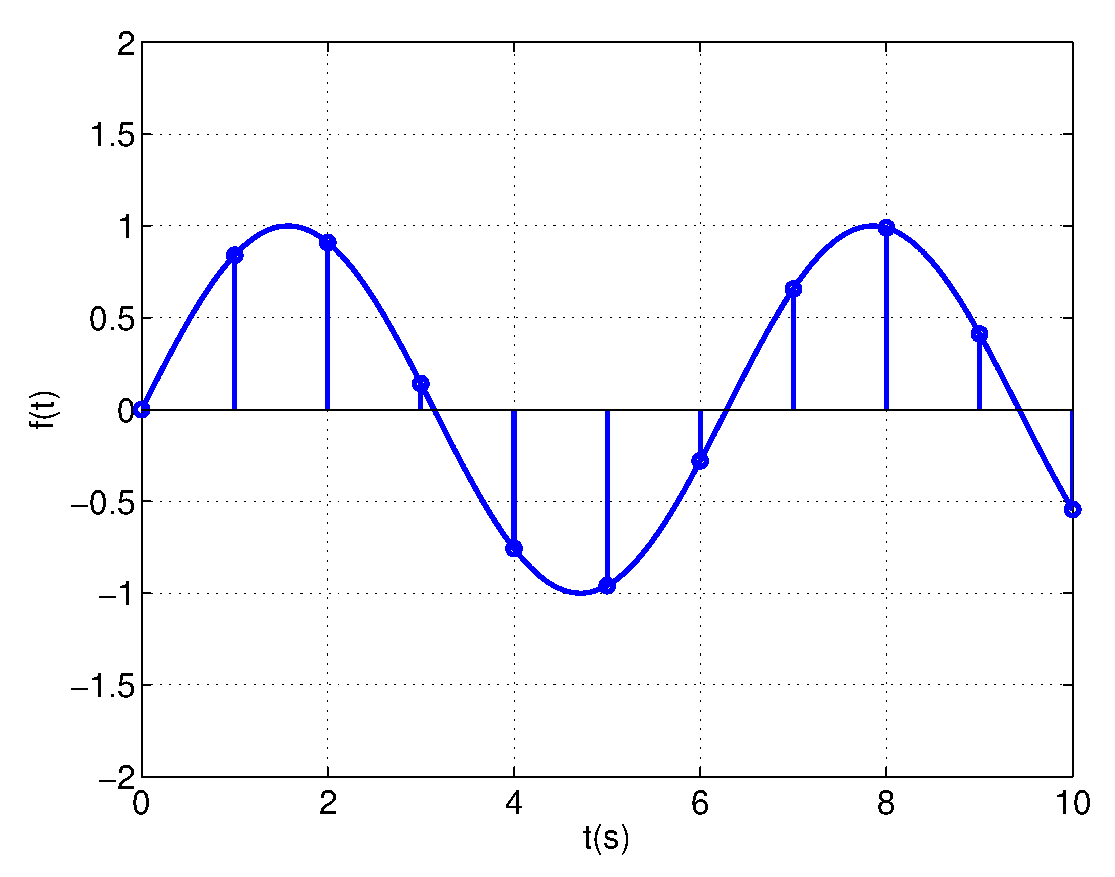
\includegraphics[width=4.5cm]{./Figures/FOHsTime0.eps}}\only<2-4|handout:0>{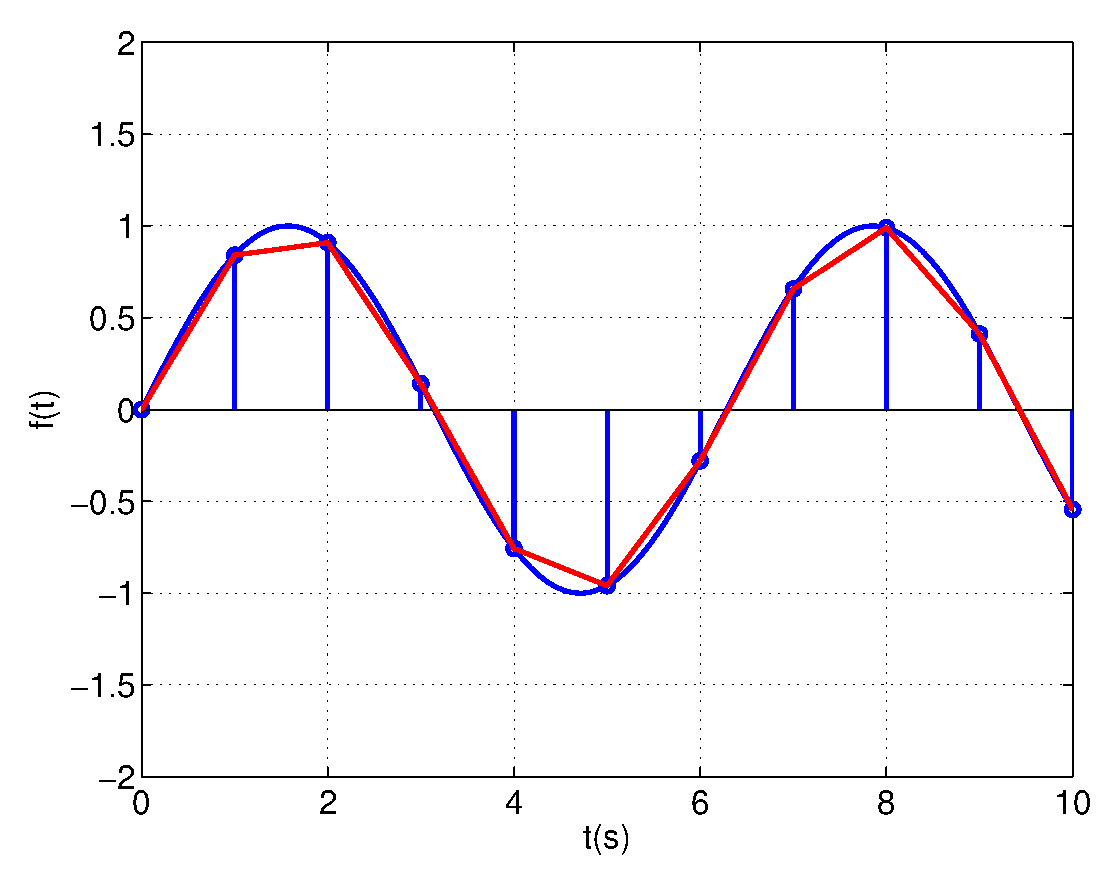
\includegraphics[width=4.5cm]{./Figures/FOHsTime1.eps}}\only<5->{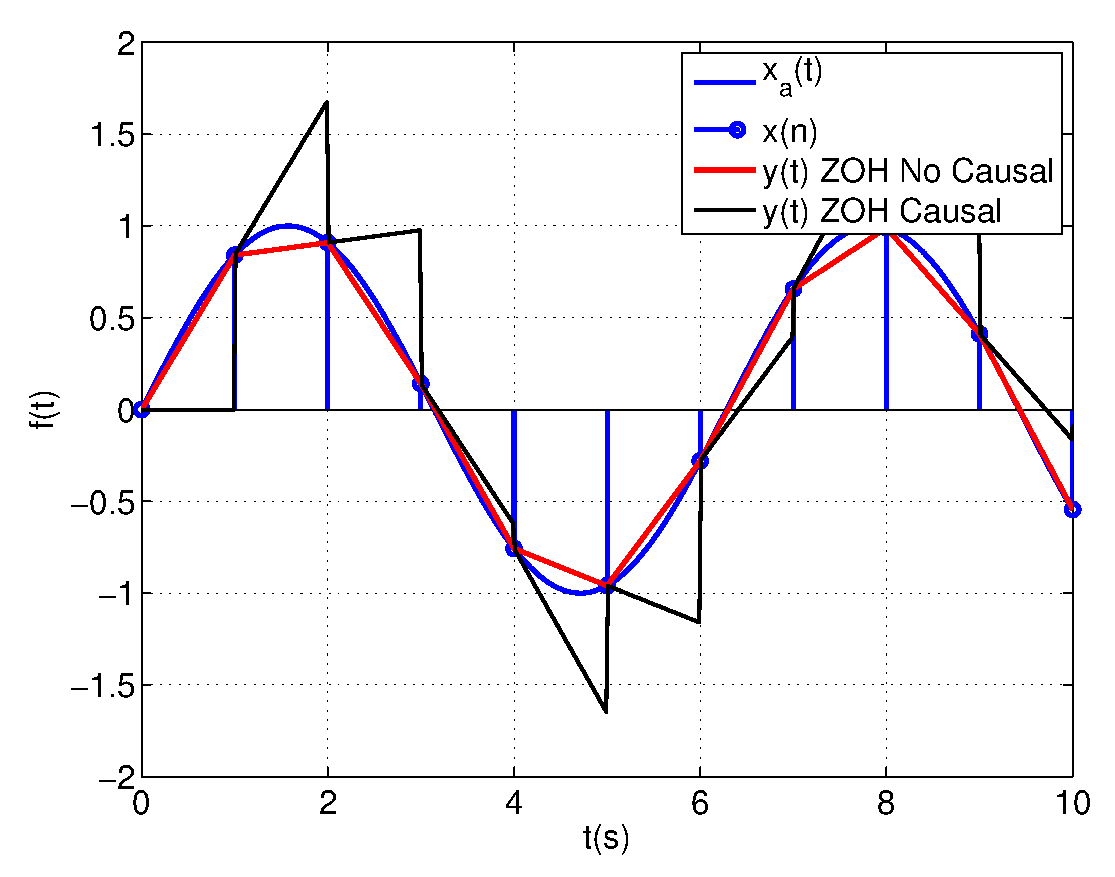
\includegraphics[width=4.5cm]{./Figures/FOHsTime.eps}}

\visible<8->{
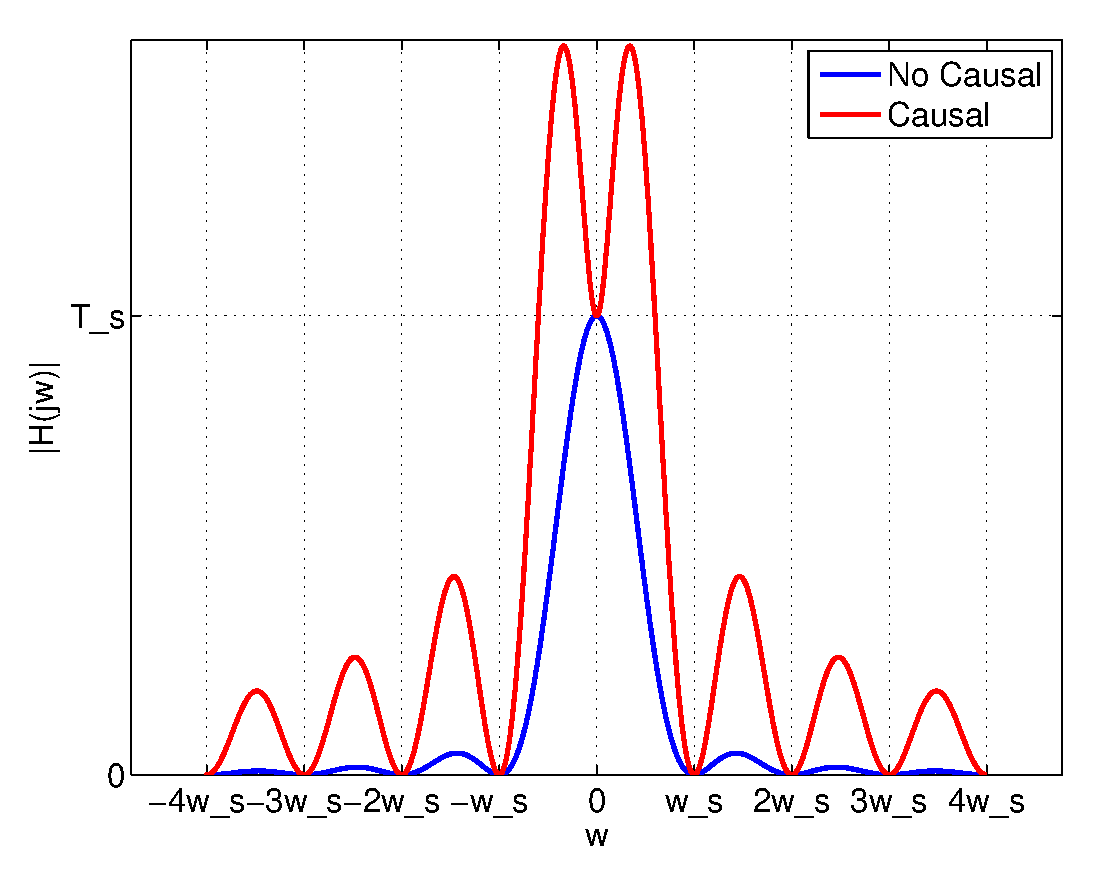
\includegraphics[width=4.5cm]{./Figures/FOHsFrec.eps}}

\end{column}
\end{columns}
\end{frame}

\section{Cuantificación y Codificación}

\begin{frame}
\frametitle{Cuantificación I}

\begin{figure}
  \centering
  \small
\scalebox{0.65}{
  \begin{psmatrix}[mnode=r,colsep=2.3,rowsep=0.1]
 [name=in]&[name=CAD]  \psframebox[fillstyle=solid,fillcolor=green,framesep=10pt,linecolor=gray,linewidth=0.4pt]{\parbox[c]{45ex}{\begin{psmatrix}[mnode=r,colsep=0.3,rowsep=0.1]
\psframebox[fillstyle=solid,fillcolor=white,framesep=10pt,linecolor=gray,linewidth=0.4pt]{\parbox[c]{10ex}{\centering Muestreador}} & \psframebox[fillstyle=solid,fillcolor=white,framesep=10pt,linecolor=gray,linewidth=0.4pt]{\parbox[c]{10ex}{\centering Cuantificador}} & \psframebox[fillstyle=solid,fillcolor=white,framesep=10pt,linecolor=gray,linewidth=0.4pt]{\parbox[c]{10ex}{\centering Codificador}}
 \end{psmatrix}
}}
& [name=out] \\
  & Conversión A/D
     
     % Connexions
     \visible<1->{\ncline[linecolor=lightgray]{->}{in}{CAD} \Bput{$x_a(t)$} \Aput{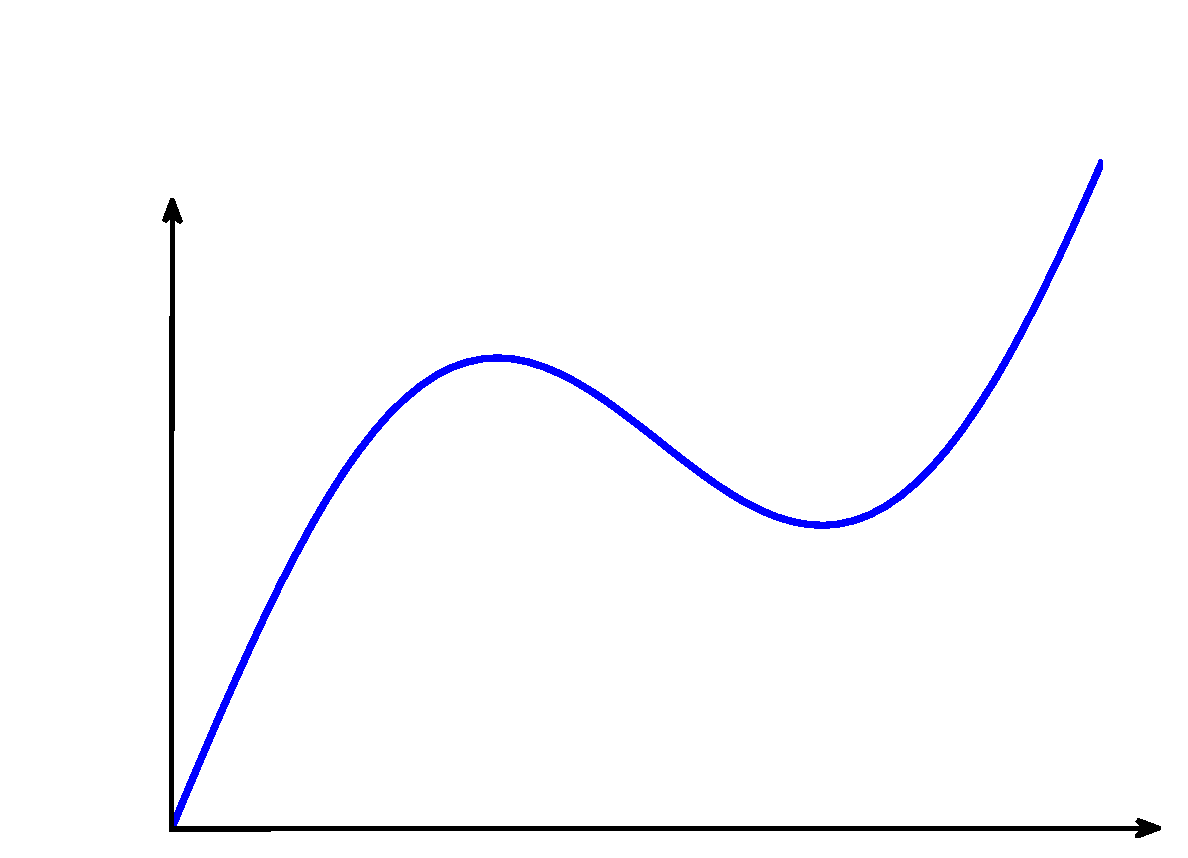
\includegraphics[width=1.5cm]{./Figures/input.eps} }} 
     \visible<1->{\ncline[linecolor=lightgray]{->}{CAD}{out} \Bput{$x_d(n)$} \Aput{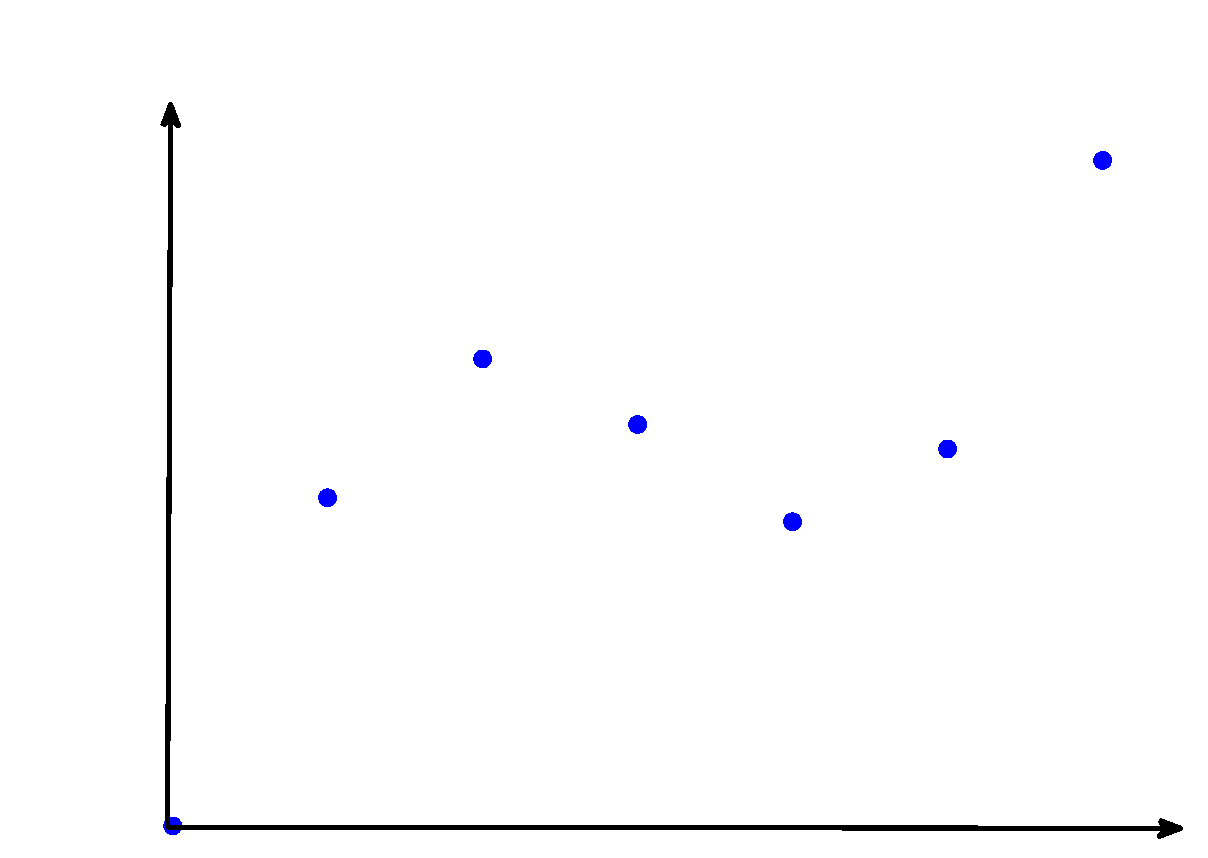
\includegraphics[width=1.5cm]{./Figures/inputD.eps} }} 
   
   \end{psmatrix}  
  }
\end{figure}

\vspace{-0.3cm}

\footnotesize
\begin{itemize}
\visible<2->{\item Una señal digital es una secuencia de números (muestras) en las que cada número se representa por un número finito de dígitos (precisión finita).}
\visible<3->{\item El proceso de convertir  una señal en tiempo discreto de amplitud constante (señal muestreada, $x(n)$) en una señal digital (doblemente discreta, $x_d(n)$) se denomina cuantificación:  \alert{ $x_d(n)=Q[x(n)]$}}
\visible<4->{\item Los niveles de cuantificación son los valores permitidos de la señal original.}
\visible<5->{\item El escalón de cuantificación o resolución $\Delta$ es  la distancia  entre dos niveles de cuantificación sucesivos.}
\begin{itemize}
\footnotesize
\visible<6->{\item El rango dinámico se define como el intervalo de valores $[x_{min},x_{max}]$ que toma la señal $x(n)$.}
\visible<7->{\item Si la señal $x(n) \in [x_{min},x_{max}]$ y existen $L$ niveles de cuantificación, $\Delta=\frac{x_{max}-x_{min}}{L-1}$.}
\visible<8->{\item Para un rango dinámico dado, si aumentamos el número de niveles aumenta la resolución (disminuye $\Delta$).}
\end{itemize} 		 
\end{itemize}

\end{frame}


\begin{frame}
\frametitle{Cuantificación II}

\footnotesize

\hspace{3cm}  \alert{ Cuantificación:  $x_d(n)=Q[x(n)]$}



\begin{itemize}
\item Tipos de cuantificación ($Q[\cdot]$):
\begin{itemize}
\footnotesize
\visible<2->{\item Redondeo: asigna cada muestra x(n) al valor del nivel de cuantificación más cercano.}
\visible<3->{\item Truncamiento: asigna cada muestra x(n) al valor del nivel de cuantificación inmediatamente inferior.}
\end{itemize}


\visible<4->{\item La diferencia entre la señal muestreada x(n) y la señal digital $x_d(n)$ se denomina error de cuantificación:  \alert{ $e_d(n)=x_d(n)-x(n)$}}

\visible<5->{\item La cuantificación es un proceso en el que se pierde información (hay un error) de forma irreversible, ya que se establece una relación entre muchos elementos (valores continuos de $x(n)$)) y uno único (nivel de cuantificación correspondiente).}


\visible<6->{\item Para un rango dinámico dado, si aumentamos el valor de niveles se reduce el error de cuantificación (ya que al disminuir $\Delta$ el error que se comete es más pequeño).}

\end{itemize}
\end{frame}

\begin{frame}
\frametitle{Ejemplo de cuantificación}

\footnotesize

\begin{itemize}
\color{olivegreen}
 \item Determinar la resoluci\'{o}n necesaria para cuantificar la señal $x(n)=0.9^n$ para representar exactamente los 10 primeros valores ($n \in [0,9]$).
 
 \visible<3->{
 \color{gray} Hay que ver cual de los x(n) necesita mayor número de dígitos: x(9) que necesita un total de 10 dígitos, por lo tanto tendríamos que cuantificarla con $\Delta=1E{-9}$}
 
 \color{olivegreen}
 \item ¿Cual es el error que se comete si se cuantifica la señal únicamente con dos dígitos?
 
 \visible<4->{
  \color{gray} Con dos dígitos, para el rango dinámico de valores del problema [0,1], tenemos que $\Delta=1E{-1}$.
  Se calcula el error como la diferencia entre el valor cuantizado (por truncamiento o redondeo) y el valor real.
 }
 \end{itemize}

\visible<2->{
 \color{gray}
\tiny
\hspace{1.5cm}\begin{tabular}{llcccc}
\hline 
 n & x(n) & $x_d(n)$ & $x_d(n)$  & $e_d(n)$  & $e_d(n)$\\
 & & Truncado & Redondeado & Truncado & Redondeado \\ \hline  
 0 &1.0   & 1.0 & 1.0  & 0.0 & 0.0\\  \hline
 1 &0.9   & 0.9 & 0.9 & 0.0 & 0.0\\  \hline
 2 &0.81 & 0.8 & 0.8  & -0.01 & -0.01 \\  \hline
 3 &0.729 & 0.7 & 0.7 & -0.029 & -0.029\\  \hline
 4 &0.6561 & 0.6 & 0.7 & -0.0561 &0.0439 \\  \hline
 5 &0.59049 & 0.5 & 0.6 & -0.09049 &0.00951\\  \hline
 6 &0.531441 & 0.5 & 0.5 & -0.031441 & -0.031441\\  \hline
 7&0.4782969 & 0.4 & 0.5 &-0.0782969 & 0.0217031\\  \hline
 8&0.43046721 & 0.4 &0.4 &-0.03046721& -0.03046721\\  \hline
 9 &0.387420489 & 0.3 &0.4 & -0.087420489 & 0.012579511\\  \hline

\end{tabular}
}

\end{frame}

%%%%%%%%%%%%%%%%%%%%%%%%%%%%%%%%%%%%%%%%%%%%%%%%%%%%%%%%%%%

\begin{frame}
\frametitle{Codificación}

\begin{figure}
  \centering
  \small
\scalebox{0.65}{
  \begin{psmatrix}[mnode=r,colsep=2.3,rowsep=0.1]
 [name=in]&[name=CAD]  \psframebox[fillstyle=solid,fillcolor=green,framesep=10pt,linecolor=gray,linewidth=0.4pt]{\parbox[c]{45ex}{\begin{psmatrix}[mnode=r,colsep=0.3,rowsep=0.1]
\psframebox[fillstyle=solid,fillcolor=white,framesep=10pt,linecolor=gray,linewidth=0.4pt]{\parbox[c]{10ex}{\centering Muestreador}} & \psframebox[fillstyle=solid,fillcolor=white,framesep=10pt,linecolor=gray,linewidth=0.4pt]{\parbox[c]{10ex}{\centering Cuantificador}} & \psframebox[fillstyle=solid,fillcolor=white,framesep=10pt,linecolor=gray,linewidth=0.4pt]{\parbox[c]{10ex}{\centering Codificador}}
 \end{psmatrix}
}}
& [name=out] \\
  & Conversión A/D
     
     % Connexions
     \visible<1->{\ncline[linecolor=lightgray]{->}{in}{CAD} \Bput{$x_a(t)$} \Aput{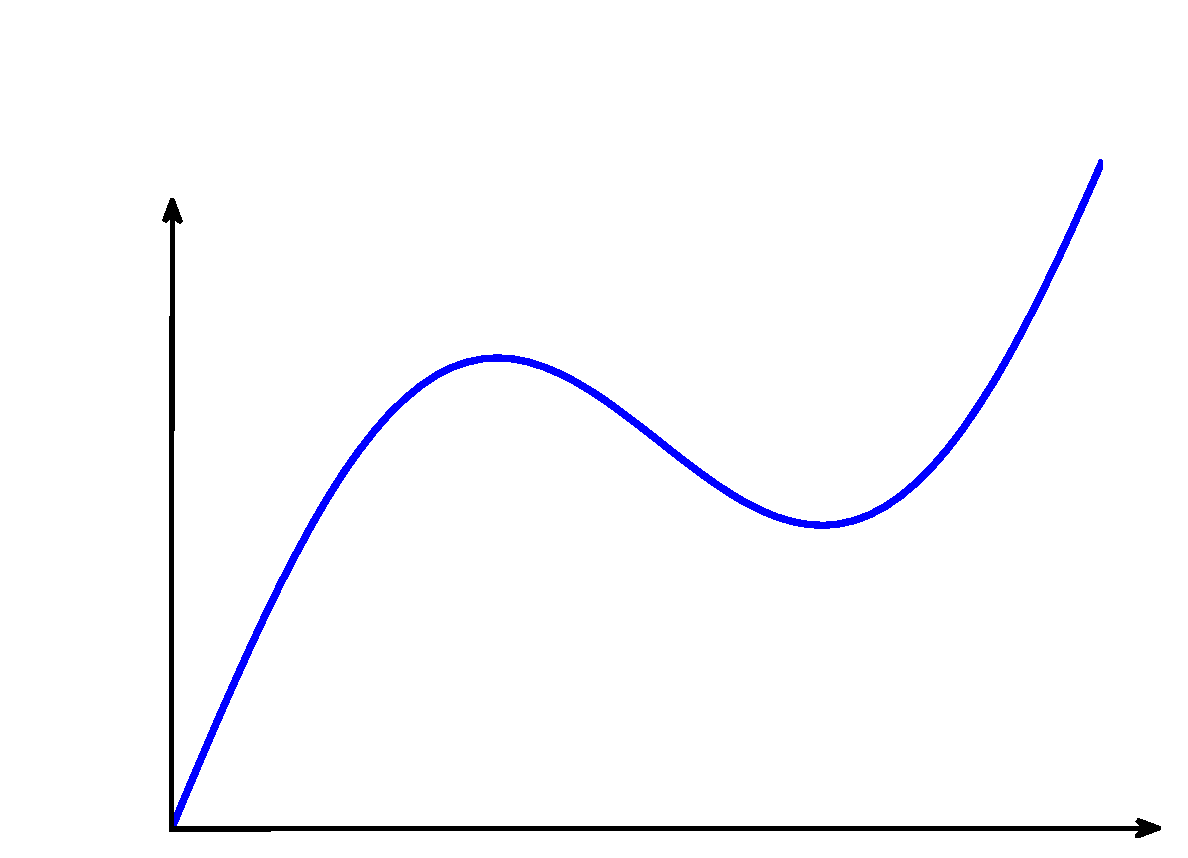
\includegraphics[width=1.5cm]{./Figures/input.eps} }} 
     \visible<1->{\ncline[linecolor=lightgray]{->}{CAD}{out} \Bput{$x_d(n)$} \Aput{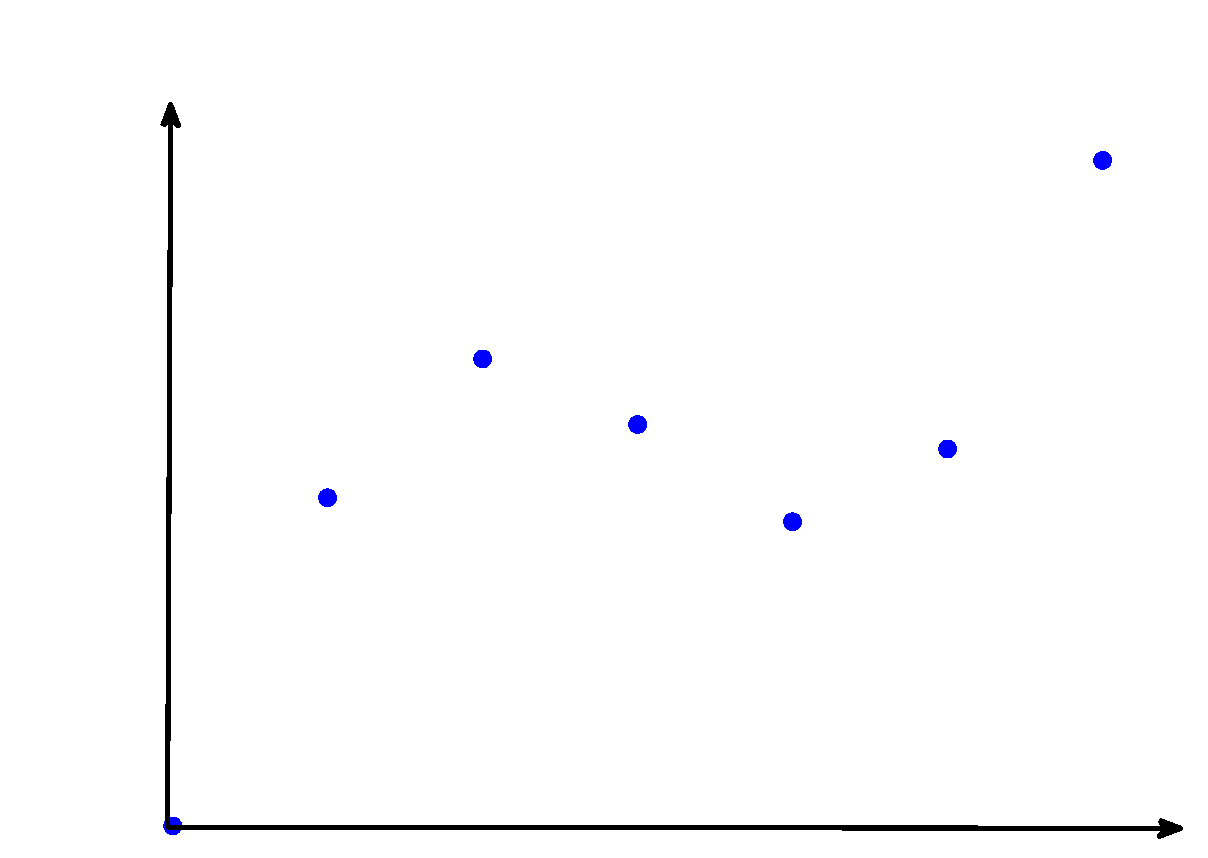
\includegraphics[width=1.5cm]{./Figures/inputD.eps} }} 
   
   \end{psmatrix}  
  }
\end{figure}

\vspace{-0.3cm}
\footnotesize

\begin{itemize}
\visible<1->{\item En el proceso de codificación se convierte la señal digital $x_d(n)$ en una cadena binaria $\{010101011\}$.}
\visible<2->{\item Si el número de niveles empleados para la cuantificación es $L$ se necesitan al menos $L$ niveles binarios  para representarla.}
\visible<3->{\item Una cadena binaria de $b$ bits permite representar $2^b$ números binarios diferentes.}
\visible<4->{\item Por lo tanto, $2^b \ge L \rightarrow b \ge log_2(L)$.

\item Es decir, el número de bits necesarios para codificar $L$ niveles es mayor o igual  $log_2(L)$.}

\vspace{0.2cm}
\visible<5->{
\hspace{-0.3cm}\color{olivegreen} Ejemplo: Calcular el número de bits necesarios para codificar 6 niveles de cuantificación.}

\visible<6->{
\color{gray}$L=6 \rightarrow log_2(L)= 2.585 \rightarrow b>=3$}


\end{itemize}


\end{frame}
  \section{Muestreo y reconstrucción de señales discretas}
  
  
  \begin{frame}
  \frametitle{Muestreo y Reconstrucción}


\vspace{-3cm}

\small

\centering 
  
  
  \begin{columns}[c]
   \hspace{-1.5cm} \begin{column}{6cm}
  \includegraphics[trim=2cm 0cm 0cm 0cm, clip=true,width=4.7cm,angle=-90]{./Figures/MuestreoD1.ps}
  \end{column}
    \begin{column}{6cm}
    \vspace{1.5cm}
      \includegraphics[trim=0cm 0cm 0cm 1cm, clip=true,width=6cm]{./Figures/MuestreoD2.ps}
  \end{column}
  \end{columns}
  
  \vspace{-2cm}
  
  			$X_p(e^{jw})=\frac{1}{N}\sum_{k=0}^{N-1} X(e^{j(w-kw_s)})$
 
  
    \end{frame}
  
    \begin{frame}
  \frametitle{Muestreo y Diezmado}
  
    \begin{columns}[T]
  \hspace{-1.5cm}\begin{column}{6cm}
  \includegraphics[trim=0cm 0cm 0cm 1cm, clip=true,width=5cm,angle=-90]{./Figures/MuestreoD3.ps}
  \end{column}
    \begin{column}{6cm}
      \includegraphics[trim=0cm 0cm 0cm 0cm, clip=true,width=5cm,angle=-90]{./Figures/MuestreoD4.ps}
  \end{column}
  \end{columns}
  
  \end{frame}

\end{document}
